\chapter{Mu2e Experiment}
\textit{
The Mu2e experiment aims to investigate the phenomenon of charged-lepton flavor violating (CLFV) neutrino-less conversion, where a negative muon transitions into an electron within the influence of a Aluminium nucleus. The experiment will measure the ratio between the conversion and the nuclear muon capture rates:
\begin{equation}\label{rmue}
R_{\mu e}=\frac{\mu^{-}+N(Z, A) \rightarrow e^{-}+N(Z, A)}{\mu^{-}+N(Z, A) \rightarrow \nu_\mu+N(Z-1, A)}
\end{equation}
The goal is to improve the current limit, set by the SINDRUM-II experiment, Ref. \cite{SINDRUMII:2006dvw}, by
four orders of magnitude and reach a SES (single-event-sensitivity) of 3 $\times$ 10$^{-17}$ on the
conversion rate, a 90\% CL of 8 $\times$ 10$^{-17}$ and a 5$\sigma$ discovery reach at 2 $\times$ 10$^{-16}$.
Mu2e is presently undergoing commissioning, integration and testing stages at the Fermilab Muon Campus, with contributions from an international collaboration. Data taking is planned to begin in 2026. This Chapter provides an overview of the employed experimental techniques and infrastructures. Fundamental bibliography for this chapter can be found in Ref. \cite{bartoszek2015mu2e}, \cite{bobbb}, \cite{Bernstein_2013}, \cite{Kargiantoulakis_2020}, \cite{universe9010054}.}
\section{Experiment concept}
A beam of negative muons, $\mu ^-$, is generated by directing a proton beam at a production target, yielding negative pions along with other mesons and hadrons. Pions, with a decay rate of more than 99.9\% due to helicity suppression, undergo $\pi ^- \rightarrow \mu ^- \bar{\nu}_\mu$ decay in flight. Accumulating sufficient statistical data within a realistic timeframe necessitates an intense muon beamline. Low-momentum secondary muons are trapped by a stopping target to form muonic atoms. Within approximately $10^{-13}$ s, a muonic atom transitions to the $1s$ state, Ref. \cite{MEASDAY2001243}. Given the brief cascading time compared to the mean muon lifetime in a muonic atom, typically around $10^{-6}$ s, instances of muon decay before reaching the ground state are negligible. The cascades emit x-ray photons, aiding in estimating the number of muons captured on the stopping target. Muonic atoms decay after a specific lifetime determined by the stopping target material. In the Mu2e experiment, an Aluminum stopping target is employed, $^{27}$Al, resulting in a lifetime of 864 ns. Muon decay occurs primarily through two processes: nuclear capture $\mu^- N \rightarrow \nu_\mu N'^* $, where $N'^*$ represents an excited magnesium nucleus ($^{27}$Mg), and muon decay-in-orbit (DIO), that is the three-body decay with neutrinos $\mu ^- N \rightarrow e^- N \nu_\mu \bar{\nu}_e$. As shown in Figure \ref{fig:muonicatom}, the ratio between these processes varies with the stopping target material. For $^{27}$Al, approximately 60.9\% of muonic atoms undergo muon nuclear capture. The remaining 39.1\% undergo muon DIO. The experiment aims to identify a third decay mode, neutrinoless muon-to-electron conversion $\mu^- N \rightarrow e^- N $. Detectors are designed to detect the signature of a single monoenergetic electron: this will be explored further in the next sections.

\section{Signals and Backgrounds}\label{sigandbkg}
\subsection{Conversion Electron Signal}
The conversion of a muon to an electron in the field of a nucleus is coherent: the muon recoils off the entire nucleus and follows two-body decay kinematics, Ref. \cite{bartoszek2015mu2e}. The mass of the nucleus is large compared to the mass of the electron, hence the recoil terms are minimal. The outgoing nucleus remains in the ground state and as a result the conversion electron (CE) is monochromatic with an energy slightly lower than the muon's rest mass:
\begin{equation}
    E_{CE} = m_\mu - E_{recoil}(A) - E_{bind}(Z) 
\end{equation}
where $m_\mu$ is the muon mass, $E_{recoil}\simeq \frac{m^2_\mu}{2 m_N}$ is the recoil energy of the target nucleus, with $m_N$ the nucleus mass, and $E_{bind}\simeq \frac{Z^2 \alpha^2 m_\mu}{2}$ is the binding energy of the $1s$ state of the muonic atom, Ref. \cite{universe9010054}. For the Mu2e stopping target material, $^{27}$Al, $E_{CE}$ = 104.97 MeV, Ref. \cite{PhysRevD.84.013006}.
\subsection{Backgrounds}\label{backgrounds}
In order to achieve a sensitivity improvement of four orders of magnitude, it is important to know all experimental backgrounds that could interfere with the process $\mu^- N \rightarrow e^- N $. Any source capable of producing 105 MeV electrons may introduce background. There are five categories of background sources, Ref. \cite{bartoszek2015mu2e}:
\begin{enumerate}
\item electrons or muons coming from cosmic rays;
\item intrinsic phenomena that vary in accordance with beam intensity, as muon Decay-in-Orbit (DIO) and Radiative Muon Capture (RMC);
\item processes that are delayed because of particles that spiral slowly down the muon beam line, such as antiprotons;
\item prompt processes where the detected electron is nearly coincident in time with the arrival of a beam particle at the muon stopping target (e.g. radiative pion capture (RPC), Pion or Muon Decay-in-Fight);
\item reconstruction errors due to accidental activities.
\end{enumerate}
The detailed discussion of these background sources will be provided below, along with the corresponding methods for mitigation. The subsequent section will focus on introducing how these mitigation techniques are applied in the Mu2e experimental design, highlighting the experiment setup.
\subsubsection{Cosmic rays}
Cosmic-ray particles, predominantly cosmic-ray muons, also contribute to the experiment background. Several mechanisms are listed here:
\begin{enumerate}
    \item muon decays occurring within or near the detectors;
    \item muons interacting with nuclei within detectors or surrounding materials;
    \item muons scattering within the detectors and being erroneously identified as electrons;
    \item muons entering the muon beamline with specific initial momentum, either interacting with collimators to produce electrons or proceeding down the muon beamline and being misidentified.
\end{enumerate}

While enhanced reconstruction algorithms can correctly identify cosmic-ray muons in certain instances, there are scenarios where signals induced by cosmic rays are indistinguishable from conversion electrons. The quantity of cosmic-ray-induced backgrounds is proportional to the duration of data collection, with the rate being experiment-specific. Detailed simulations estimated that in the Mu2e experiment, conversion-like signals generated by cosmic rays occur approximately once per day, potentially overwhelming actual conversion signals, Ref. \cite{CRVposter}. Mitigation involves employing a combination of active veto and shielding within the experiment. As shown in Section \ref{CRV}, a high-efficiency veto system is capable of effectively reducing cosmic-ray-induced backgrounds to an acceptable level.
\subsubsection{Intrinsic Backgrounds}
The intrinsic backgrounds in the experiment originate from two physics processes: muon decay-in-orbit (DIO) and radiative muon capture (RMC). In this context, $intrinsic$ denotes that the rates of these backgrounds are directly correlated with the number of muons captured on the stopping target.
\paragraph{Muon Decay-in-Orbit}
Electrons energy coming from the three body decay of a free muon, $\mu^- \rightarrow e^- \bar{\nu}_e \nu_\mu$, is described by the Michel Spectrum. The differential decay rate can be computed, Ref. \cite{michel}:
\begin{equation}
    \frac{\text{d}\Gamma_{\text{free}}}{\text{d}x}= \frac{G^2_F m^5_\mu}{192 \pi^3}x^2(6-4x+\frac{\alpha}{x}f(x)) 
\end{equation}
where $x=\frac{2 E_e}{m_\mu}$, $0\leq x\leq 1$, $G_F$ is the Fermi constant, $\alpha$ is the fine-structure constant, $m_\mu$ is the muon mass, $E_e$ is the electron energy and $f (x)$ represents a complicated radiative correction term, described in Ref. \cite{PhysRev.113.1652}. 
As shown in Figure \ref{fig:linearscalemichel}, the spectrum exhibits a peak energy at 52.8 MeV, constituting half of the muon rest energy  or the energy of the searched conversion electron. However, the presence of an Al nucleus allows the electron to interact with it, exchanging momentum and resulting in a maximum possible energy, $endpoint$ $energy$, that closely matches that of the conversion electron (negligible neutrino energy in this scenario). The difference between the two energy spectra, one neglecting the nuclear recoil and the other influenced by the Al nucleus, is illustrated in Figure \ref{fig:micheldiff}. Figure \ref{fig:logscalemichel} presents a more detailed examination of the high-energy range of the spectrum. When the electron energy $E_e \ \geq$ 85 MeV, the dominant term at the leading order scales with $(E_{\mu e} - E_e)^5$, Ref. \cite{PhysRevD.84.013006}, resulting in a low rate within the energy range very close to the endpoint. However, in actual experimental conditions, due to uncertainties in reconstructions and the energy loss of particles when interacting with stopping targets or detector materials, the monoenergetic conversion electrons tend to be reconstructed with a left-skewed energy distribution, with a full width at half maximum (FWHM) approximately on the order of 1 MeV, Ref. \cite{gaponenko}, as shown in Figure \ref{fig:sensitivity}. Consequently, the high-energy electrons originating from muon DIO and the conversion electrons become indistinguishable. To limit the DIO background, Mu2e detectors are designed to be blind to the majority of low-energy electrons. A particle tracking detector with high momentum resolution also helps to reduce background noise, which will be explored in next sections.
\begin{figure}[!h]
     \begin{subfigure}[b]{0.4\linewidth}
         \centering
         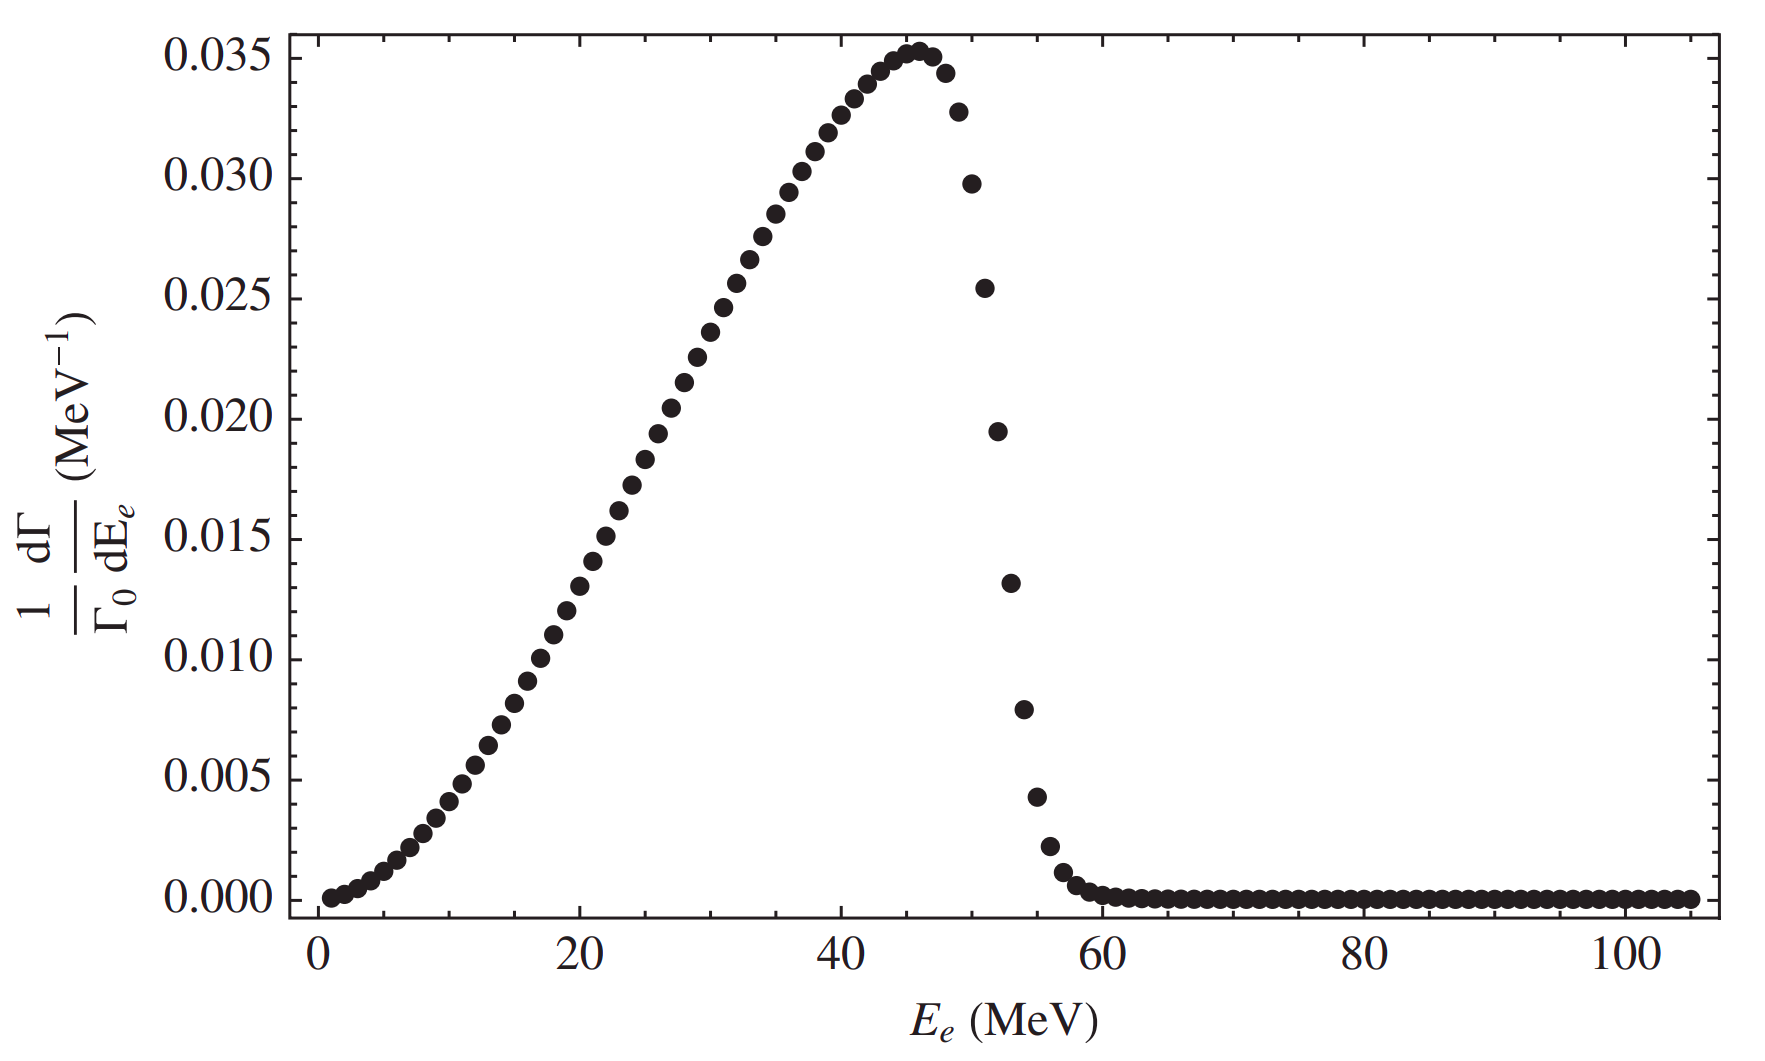
\includegraphics[scale = 0.18]{images/chapter2/Screenshot_20240222_175415.png}
         \subcaption{Linear scale.}
         \label{fig:linearscalemichel}
     \end{subfigure}
     \begin{subfigure}[b]{0.7\linewidth}
         \centering
         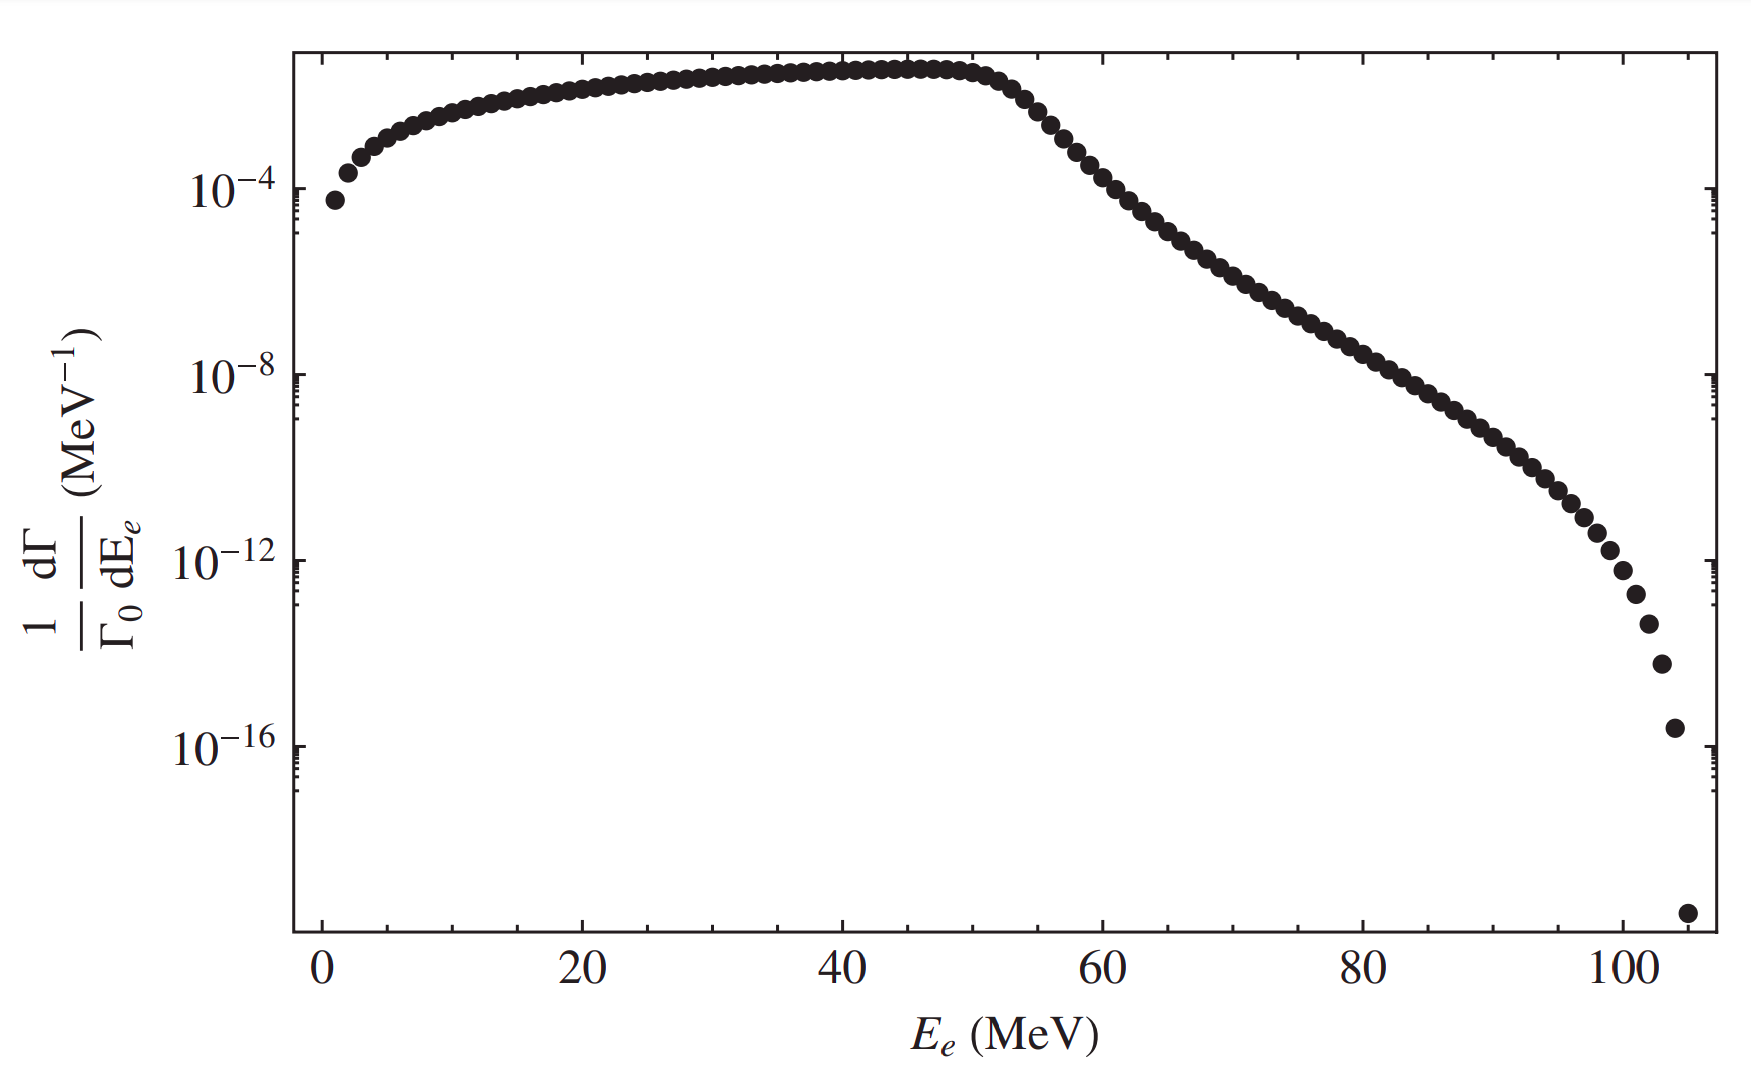
\includegraphics[scale = 0.18]{images/chapter2/Screenshot_20240222_175446.png}
         \subcaption{Logarithmic scale.}
         \label{fig:logscalemichel}
     \end{subfigure}
     \caption{Electron spectrum for aluminum, Ref. \cite{PhysRevD.84.013006}.}
        \label{fig:michel}
\end{figure}

\begin{figure}[!h]
\centering
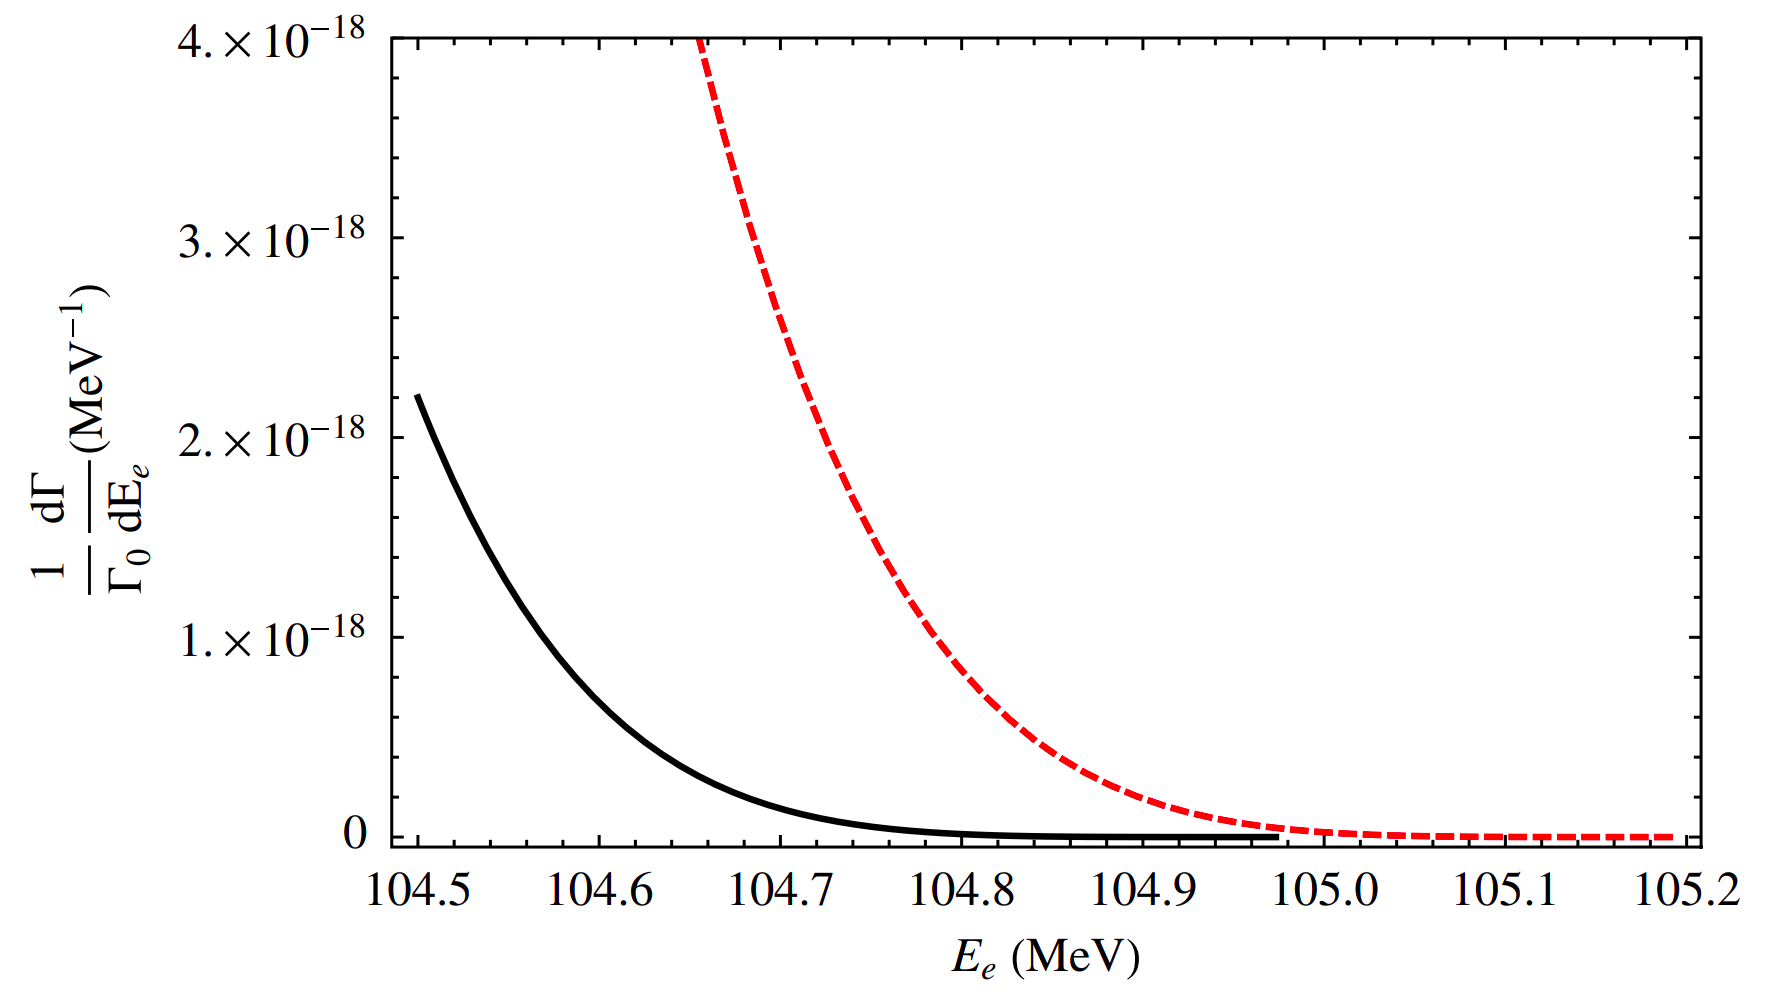
\includegraphics[width =0.55\textwidth]{images/chapter2/Screenshot_20240222_175644.png}
\caption{The electron energy spectrum near to the endpoint. The black line represents the Michel spectrum when neglecting nuclear recoil, while the red dashed line takes into consideration the recoil of the Aluminum nucleus, Ref. \cite{PhysRevD.84.013006}.}
\label{fig:micheldiff}
\end{figure}
\paragraph{Radiative Muon Capture}

The Radiative muon capture (RMC) process differs from ordinary muon nuclear capture by producing an additional photon. In the process $\mu^- N \rightarrow\gamma \nu_\mu N'^* $, the photon can either be real or virtual. The photon, interacting with matter or undergoing pair production, can produce electrons with energies close to $E_{CE}$, introducing background signals to the experiment. The emitted photon's energy follows a spectrum, with its maximum energy, denoted as the kinematic limit $k_{max}$, determined by the equation (Ref. \cite{bartoszek2015mu2e}):

\begin{equation}
k_{max} = m_\mu c^2 - |E_b| - E_{rec} - \Delta M ,
\end{equation}

where $E_b$ represents the muon binding energy on the initial nucleus, $E_{rec}$ denotes the recoil energy of the daughter nucleus and $\Delta M$ is the rest energy difference between the final and initial nuclides. This formula neglects higher order nuclear effects. RMC can be effectively mitigated in the Mu2e experiment by selecting Aluminum as the stopping target material. The stopping target is selected so that the daughter nuclide of a muon-capture process of any kind is heavier than the original nuclide. For aluminum, the RMC endpoint energy is 101.9 MeV, approximately 3.1 MeV below the conversion electron energy, Ref. \cite{bartoszek2015mu2e}. The planned FWHM of the conversion peak is around 1 MeV, therefore the RMC background will be outside the signal region. However, the RMC background might distort the DIO spectra in the 80-100 MeV range, making it difficult to extrapolate to the endpoint. Determining the RMC background from the data will be a crucial part of the experiment.
\subsubsection{Prompt Processes}
This type of background sources can generate electrons at roughly the same time as the entering beam particles. There are four primary sources: radiative pion capture (RPC), pion decay-in-flight ($\pi$-DIF), muon decay-in-flight ($\mu$-DIF) and beam electrons.
\paragraph{Radiative Pion Capture}
The secondary muon beam carries a considerable quantity of pions.  It is not excluded that some pions can reach the stopping target. Pions, when captured in materials, can produce a high-energy photon, i.e. $\pi^- N(A,Z) \rightarrow \gamma N ^* (A,Z-1)$. This phenomenon, called radiative pion capture, is observed in approximately 2\% of pions captured in Aluminum, Ref. \cite{PhysRevC.5.1867}. Similar to RMC, the photon can internally convert into an electron-positron pair or emit an on-shell photon, leading to pair production. The external pair-production depends on the thickness of the material. The resulting electrons can contribute to the experiment background. Despite its similarity to RMC, RPC is more challenging background to suppress due to the fact that the endpoint of the energy spectrum of photons, and consequently the resulting electrons, is not constrained by the rest energy of the muon. The mass of a pion is 139.6 MeV, which is much higher than the conversion energy. Consequently, there exists no energy separation between the search range for conversion electrons and the electron energy spectrum originating from RPC photons. The SINDRUM II results were limited by the pion-induced background and also by the low intensity of its muon beam, Ref. \cite{SINDRUMII:2006dvw}. SINDRUM II employed a primary proton beam with a frequency of one pulse every 19.75 ns, lasting approximately 0.3 ns. This interval between pulses was shorter than the 26 ns lifetime of pions, Ref. \cite{zyla}, ensuring a consistent pion flux. To mitigate RPC, SINDRUM II employed a degrader to suppress pions and a veto counter in the beam, resulting in less than 1 out of 109 pions reaching their target. However, given the more intense beam, the Mu2e experiment has to change the approach. Mu2e employs a pulsed proton beam. Given their brief lifetime, nearly all pions decay or interact with materials shortly after the pulse of the proton beam. The RPC background can be suppressed by opening a live window for conversion electron search at a right time. One important point to note is that in the event of protons coming out of the beam pulse, out-of-time, the resultant pions could still contribute to RPC background. Consequently, it is important for the pulsed beam to achieve a high extinction level, ensuring that the ratio of out-of-time to in-time RPC remains below a specified threshold. Further elaboration on the pulsed beam used in Mu2e will be provided in Section \ref{accel}.
\paragraph{$\pi$-DIF and $\mu$-DIF}
The decay-in-flight of the pion ($\pi$-DIF) and the decay-in-flight of the muon ($\mu$-DIF) exhibit quite similar characteristics. Free pions and muons can undergo electron decay while transitioning from the production target to the stopping target, through the processes $\mu^- \rightarrow e^- \nu_\mu \bar{\nu}_e$ and $\pi^- \rightarrow e^- \bar{\nu}_e$. In the center-of-mass frame of the initial particles, electrons originating from the first process exhibit an energy spectrum that reaches an endpoint of 52.8 MeV, while those from the second process have a consistent energy of approximately 70 MeV. As the pions and muons move at relativistic velocities, the energies (and momenta) of the resultant electrons are boosted. For instance, a muon with a momentum of around 79 MeV/c or a pion with momentum close to 70 MeV/c can generate an electron with an energy of 105 MeV, Ref. \cite{bartoszek2015mu2e}. Implementing a pulsed proton beam and employing a delayed live window can help suppress background from $\pi$-DIF and $\mu$-DIF events. Particles with sufficient momentum to boost the daughter electrons to the concerning energies move quickly along the muon beamline and are gone by the time the live search window begins, Ref. \cite{bobbb}. In addition, the shape of the Mu2e detectors contributes to mitigation.
\paragraph{Beam electrons}\label{beamelectrons}
Other mechanisms generate electrons, both at the production target and along the muon beamline. For instance, neutral pions formed at the production target can decay in two photons, after which the photons can either create electron-pairs or interact with nearby materials to generate electrons. Other beam particles can decay or interact at any point before the muon stopping target, producing electrons with energy equal to $E_{CE}$. These sources of background are colled beam electrons and it is possible to reduce them through the pulsed beam and the delayed live window. Moreover, Mu2e uses a set of solenoids to generate a magnetic field across the muon beamline and in the area of the stopping target and detectors. A charged particle follows a spiral trajectory when a magnetic field is applied, where the size and shape of the spiral are determined by the particle's electric charge and its parallel and perpendicular to magnetic field components of momentum. This brings to the installation of collimators along the muon beamline to suppress the number of high-momentum particles exceeding 100 MeV/c, Ref. \cite{bartoszek2015mu2e}. Moreover, the magnetic field is designed with a gradient in proximity of the stopping target. This gradient effectively divides the paths of conversion electrons from those originating upstream, unless they undergo scattering within the stopping target, Ref. \cite{bobbb}. Solenoid system and the magnetic field will be deeply explored in Section \ref{setup}.
\subsubsection{Delayed processes from antiprotons}
Protons, at a given threshold, can generate antiprotons within the production target. This occurs through the process of antiproton production: $pp \rightarrow ppp\bar{p}$. The minimum kinetic energy of the initial proton beam can be found applying 4-momentum conservation principles to the system. 
If we consider that all four particles in the final state are at rest in the center of mass frame, the minimum kinetic energy needed for $p\bar{p}$ production can be found, which is approximately $6 m_pc^2 \sim 5.6$ GeV, where $m_p$ is the mass of the proton. In an ideal scenario, maintaining the beam energy below this threshold could enable us to avoid this background in the experiment. Unfortunately, the Mu2e proton beam goes beyond the threshold for antiproton production. The antiprotons are long-lived and massive. Antiprotons with momenta below 100 MeV/c travel at speeds less than 0.1$c$, requiring several $\mu$s to spiral from the production target to the stopping target, Ref. \cite{bartoszek2015mu2e}. They have the correct charge and momentum to pass through the collimators placed between the production target and the stopping target. Annihilating or undergoing interactions with other materials, they have the capability to release a substantial amount of energy, generating numerous secondary electrons. The time delay connected with these interactions significantly exceeds the muon lifetime, leading to a continual flow of antiprotons reaching the stopping target. The pulsed beam and the delayed live window fail to suppress the antiproton background. The best approach is to prevent the antiprotons from reaching the region where the stopping target is located. A thin absorber is positioned in the muon beamline to capture the antiprotons. Its design was developed to find a compromise between increasing antiproton absorption and decreasing muon beam loss.
\subsubsection{Accidental activity}
This final background category arises not from the physical interactions of a specific particle, but rather from the accidental reconstruction of extra events in the detectors, miming conversion-like signals. During the muon-capture process, nuclei in excited states can expel protons, neutrons and photons. These expelled protons have high ionization potential, producing large signals in the detectors and increasing the likelihood of reconstruction errors. Additionally, other coincidences, such as multiple muon decay-in-orbit occurring in close succession, can also contribute to reconstruction errors. To suppress the flux of protons from the muon-capture process reaching the detectors, additional polyethylene absorbers are used to surround the stopping target in the Mu2e experiment. A systematic uncertainty is evaluated as part of the background analysis to take into account these accidental events.

\subsection{Backgrounds estimates and Signal Sensitivity}
Mu2e run plan is divided in two different phases. Run I will take place in 2026, before a 2 years shutdown due to the planned accelerator upgrade for the long baseline neutrino program. In Run I phase one, a low intensity proton beam, $1.6 \times 10^7$ protons/pulse, will be used. In Run I phase two, the mean intensity will be increased up to $3.9 \times 10^7$ protons/pulse. The total number of stopped muons will be $6 \times 10^{16}$, corresponding to the 10\% of the number required to satisfy the Mu2e goals in the complete data-taking. As discussed in Ref. \cite{universe9010054}, the discovery $R_{\mu e}$, Ref. \ref{rmue}, corresponding to a 50\% probability of observing the conversion signal at a 5$\sigma$ significance level is $R_{\mu e}^{5 \sigma}= 1.2 \times 10^{-15} $. Reaching the 5$\sigma$ significance level requires observing 5 $\mu\rightarrow e$ events in the two-dimensional search window 103.60 < $p$ < 104.90 MeV/c, 640 < $T_0$ < 1650 ns. One of the
parameters characterizing the sensitivity of an experiment to a process of interest is its
single event sensitivity (SES), defined as:
\begin{equation}
    SES \equiv \frac{1}{N_{POT} \cdot P_{\mu \ stop} \cdot \epsilon_{CE} \cdot BR_{capture}}
\end{equation} 
$N_{POT}$ means the number of protons on target in the experiment, $P_{\mu \ stop}$ is the number of muons stopped on target per proton, $\epsilon_{CE}$ is the conversion electron acceptance, which is a product of detector efficiency (dependent on the momentum signal region) and fraction of muons interacting in the live time window and $BR_{capture}$ is the branching ratio of muon captures, which is 60.9\%. The optimized Mu2e signal window corresponds to a SES of $2.4 \times 10^{-16}$. The background estimates after the sensitivity optimization are summarized in Table \ref{tab:summarybkg}, resulting in a total background of approximately $\sim$ 0.1 event/year. Figure \ref{fig:sensitivity} shows the momentum and time distributions for CE signal and background processes corresponding to the optimized signal window for Run I. A detailed analysis and estimate of the Mu2e expected backgrounds for Run I can be found in Ref. \cite{universe9010054}.
\begin{center}  
\begin{table}[!h]
\centering
\renewcommand{\arraystretch}{1.2}
\begin{tabular}{| c | c |}
\hline
\textbf{Channel} & \textbf{Mu2e Run I}\\
\hline
SES & 2.4 $\times \ 10^{-16}$ \\
\hline
Cosmic rays & 0.046 $\pm$ 0.010 (stat.) $\pm$ 0.009 (syst.) \\
DIO & 0.038 $\pm$ 0.002 (stat.) $ ^{+ \ 0.025} _{- \ 0.015}$ (syst.)\\
Antiprotons & 0.010 $\pm$ 0.003 (stat.) $\pm$ 0.010 (syst.) \\
RPC in-time & 0.010 $\pm$ 0.002 (stat.) $ ^{+ \ 0.001} _{- \ 0.003}$ (syst.)\\
RPC out-of-time & (1.2 $\pm$ 0.1  (stat.) $ ^{+ \ 0.1} _{- \ 0.3}$ (syst.)) $\times$ $10^{-3}$ \\
RMC & $<$ 2.4 $\times$ $10^{-3}$ \\
Decays in flight & $<$ 2 $\times$ $10^{-3}$ \\
Beam electrons & $<$ 1 $\times$ $10^{-3}$ \\
\hline
Total &  0.105 $\pm$ 0.032\\
\hline
\end{tabular}
\caption{Summary of the several background sources to the conversion electron search as expected in Mu2e Run I,  Ref. \cite{universe9010054}. The table also shows the corresponding single event sensitivity (SES). This is is defined as the $R_{\mu e}$ ratio when there is one signal event.}
\end{table}\label{tab:summarybkg}
\end{center}
\begin{figure}[!h]
\centering
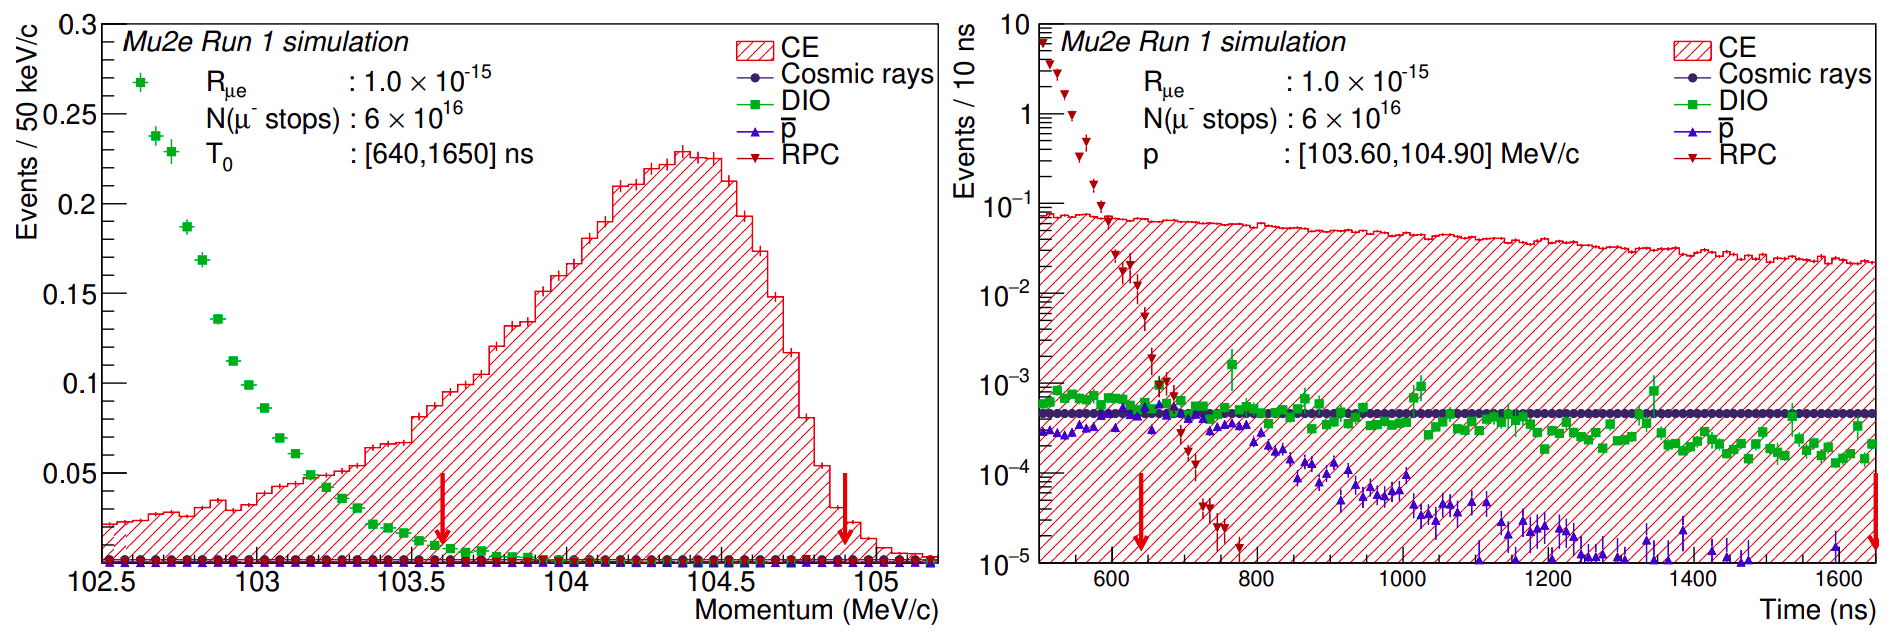
\includegraphics[width =0.93\textwidth]{images/chapter2/Screenshot_20240225_102708.png}
\caption{Left: Momentum distribution of the conversion electron signal and expected backgrounds. Right: Time distribution of the conversion electron signal and expected backgrounds. The arrows show the signal region selected for the analysis,103.60 $< \ p \ < $ 104.90 MeV/c and 640 $< \ T_0 \ < $ 1650 ns, Section \ref{pulsedprotonbeam}. The $CE$ signal distributions correspond to $R_{\mu e} = 1 \times 10^{-15}$, Ref. \cite{universe9010054}.}
\label{fig:sensitivity}
\end{figure}
\section{Experimental setup}\label{setup}
Figure \ref{fig:mu2escheme} shows a schematic overview of the Mu2e experiment, illustrating the trajectory of the pulsed proton beam directed towards the production target indicated by the red arrow. The experiment uses a solenoid system to generate magnetic fields essential for its operations. The Production Solenoid (PS) surrounds the production target, while further downstream, the Transport Solenoid (TS) provides the magnetic field for the muon beamline. The TS, configured in an S-shape, incorporates collimators and proton absorbers strategically positioned to minimize experimental backgrounds. The stopping target is located at the beginning of the Detector Solenoid (DS). Proton absorbers surround the stopping target, not shown in the figure. The Tracker and the Calorimeter are housed in the DS, enabling momentum and energy measurements, respectively. Additionally, a Stopping Target Monitor (STM) positioned downstream at the DS's end, not shown, monitors the stopping target's condition and estimates the captured muon count. Not shown in the figure is the Mu2e Cosmic Ray Veto (CRV) system: it surrounds the DS and half of the TS. In next sections, a more detailed description of systems of the Mu2e experiment will be given.
\begin{figure}[!h]
\centering
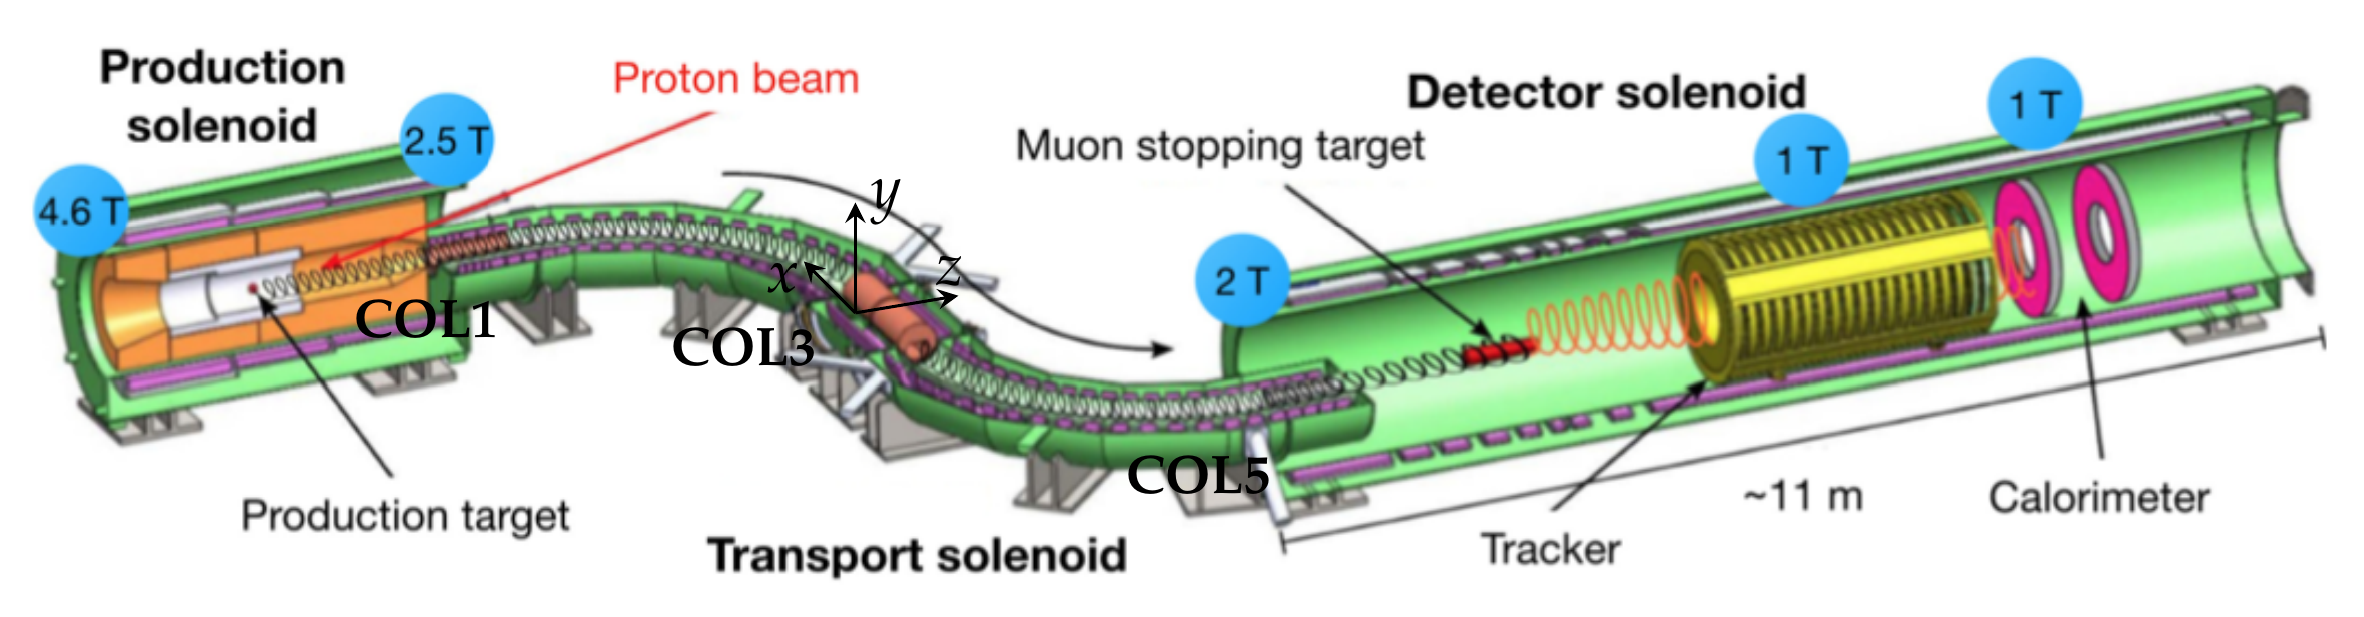
\includegraphics[width =\textwidth]{images/chapter2/Screenshot_20240301_143105.png}
\caption{Schematic view of the Mu2e apparatus. The center of the Mu2e reference frame is located at the COL3 collimator center, its y-axis points upwards, the z-axis is parallel to the DS axis and points downstream, and the x-axis completes the right-handed reference frame, Ref. \cite{universe9010054}.}
\label{fig:mu2escheme}
\end{figure}
\section{Accelerator system and Proton Beam}\label{accel}
\subsection{Pulsed Proton Beam}\label{pulsedprotonbeam}
As previously discussed in Section  \ref{backgrounds}, the Mu2e experiment employs a pulsed proton beam to reduce background from prompt processes, as pion capture. The 8 GeV, 8 kW beam originates from the Fermilab Booster, Ref. \cite{PhysRevAccelBeams.20.111003}. A pulsed beam with a 1695 ns gap between two pulses is needed. Figure \ref{fig:accell} illustrates the Fermilab accelerator facilities involved in generating and delivering the pulsed proton beam. The Fermilab Booster delivers 8 GeV protons in 20 batches throughout a 1.4 s Main Injector cycle at 15 Hz, as shown in Figure \ref{fig:deliver}. Thus, the accelerator timeline is described using a fundamental time unit of 1 tick that corresponds to 66.7 ms.

\begin{figure}[!h]
     \begin{subfigure}[b]{0.4\linewidth}
         \centering
         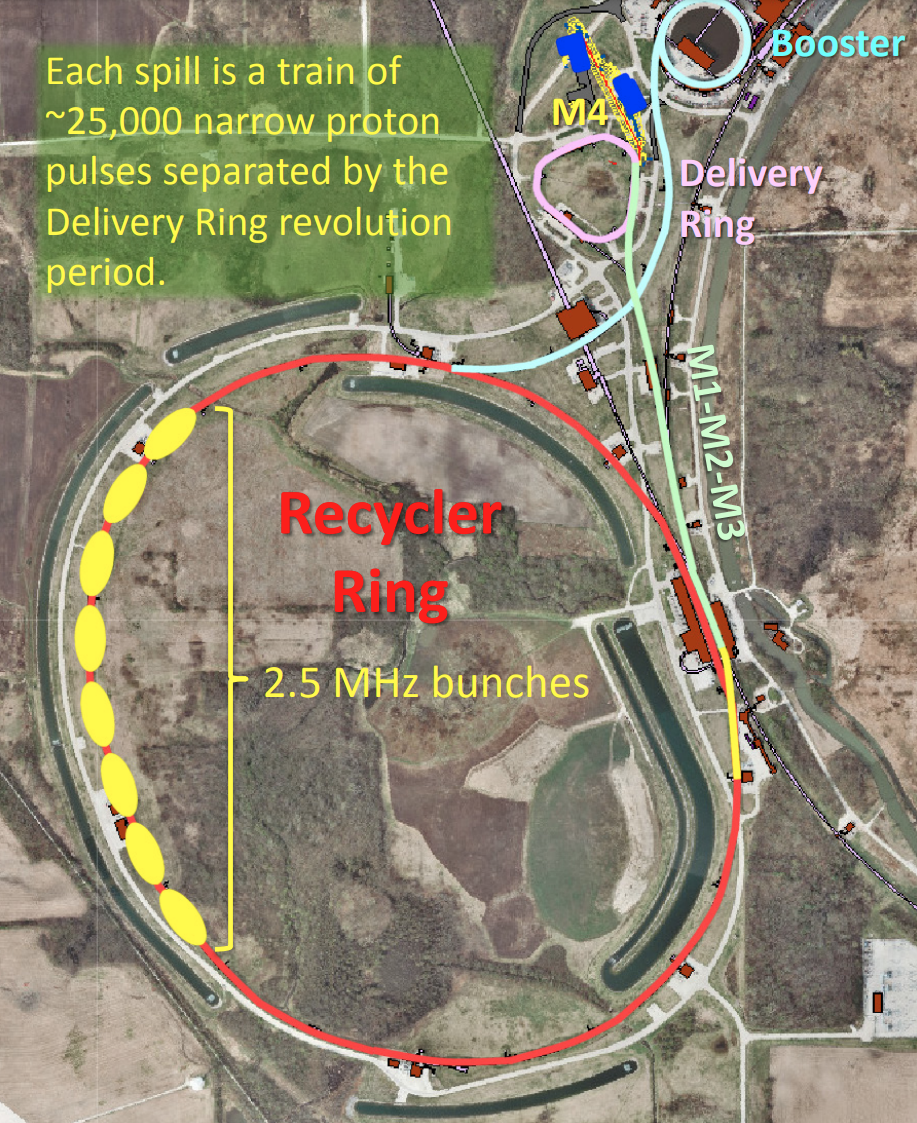
\includegraphics[scale = 0.3]{images/chapter2/Screenshot_20240301_151449.png}
         \subcaption{\centering Fermilab accelerator facilities involved in producing and delivering the pulsed proton beam.}
         \label{fig:accell}
     \end{subfigure}
     \begin{subfigure}[b]{0.7\linewidth}
         \centering
         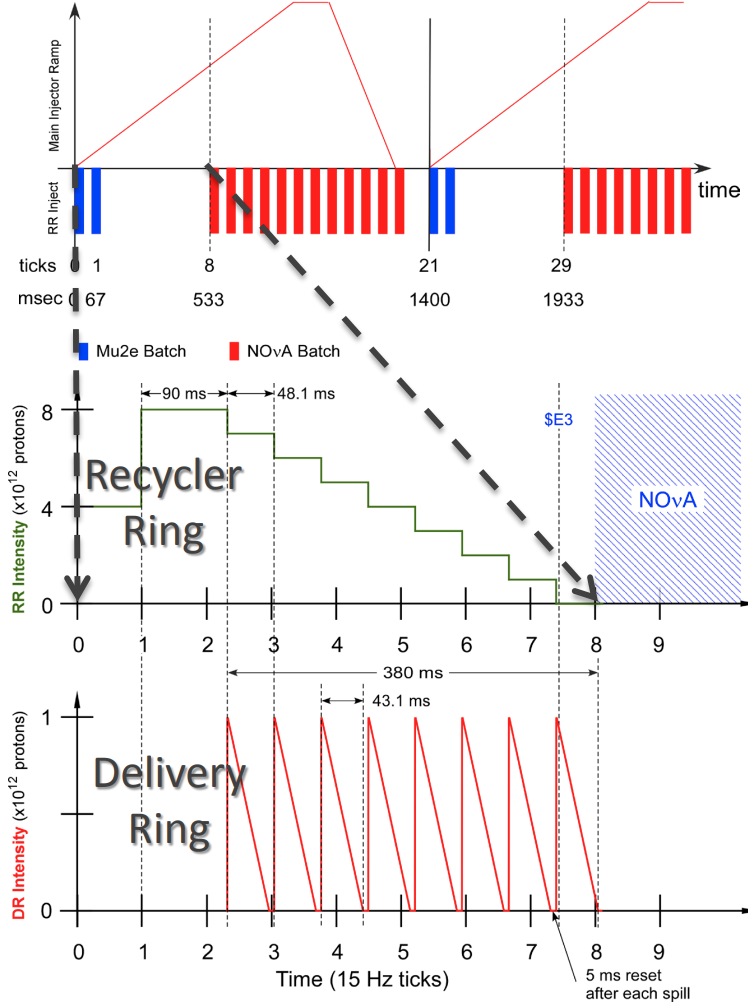
\includegraphics[scale = 0.39]{images/chapter2/Screenshot_20240301_151418.png}
         \subcaption{\centering Proton beam delivery to Mu2e.}
         \label{fig:deliver}
     \end{subfigure}
     \caption{Pulsed proton beam delivery, Ref. \cite{accelerator}.}
        \label{fig:three graphs1}
\end{figure}
The two Mu2e batches, represented by the two blue bars at ticks 1 and 2, are injected into the Recycler Ring, each containing $4 \times 10^{12}$ protons. The protons from these batches are reorganized within the Recycler using a 2.5 MHz radio frequency (RF) system into 8 bunches. These bunches are then extracted individually from the Recycler and transported to the Delivery Ring every 48.1 ms, as shown in the middle part of Figure \ref{fig:deliver}. Once inside the Delivery Ring, a single bunch of $1 \times 10^{12}$ protons undergoes gradual extraction. This process results in the extraction of a small fraction of the bunch per revolution, delivered to the Mu2e experiment. The complete bunch is extracted over a span of 43.1 ms, across $\sim$25000 turns around the Delivery Ring, as shown in the bottom part of Figure \ref{fig:deliver}.
\begin{figure}[!h]
\centering
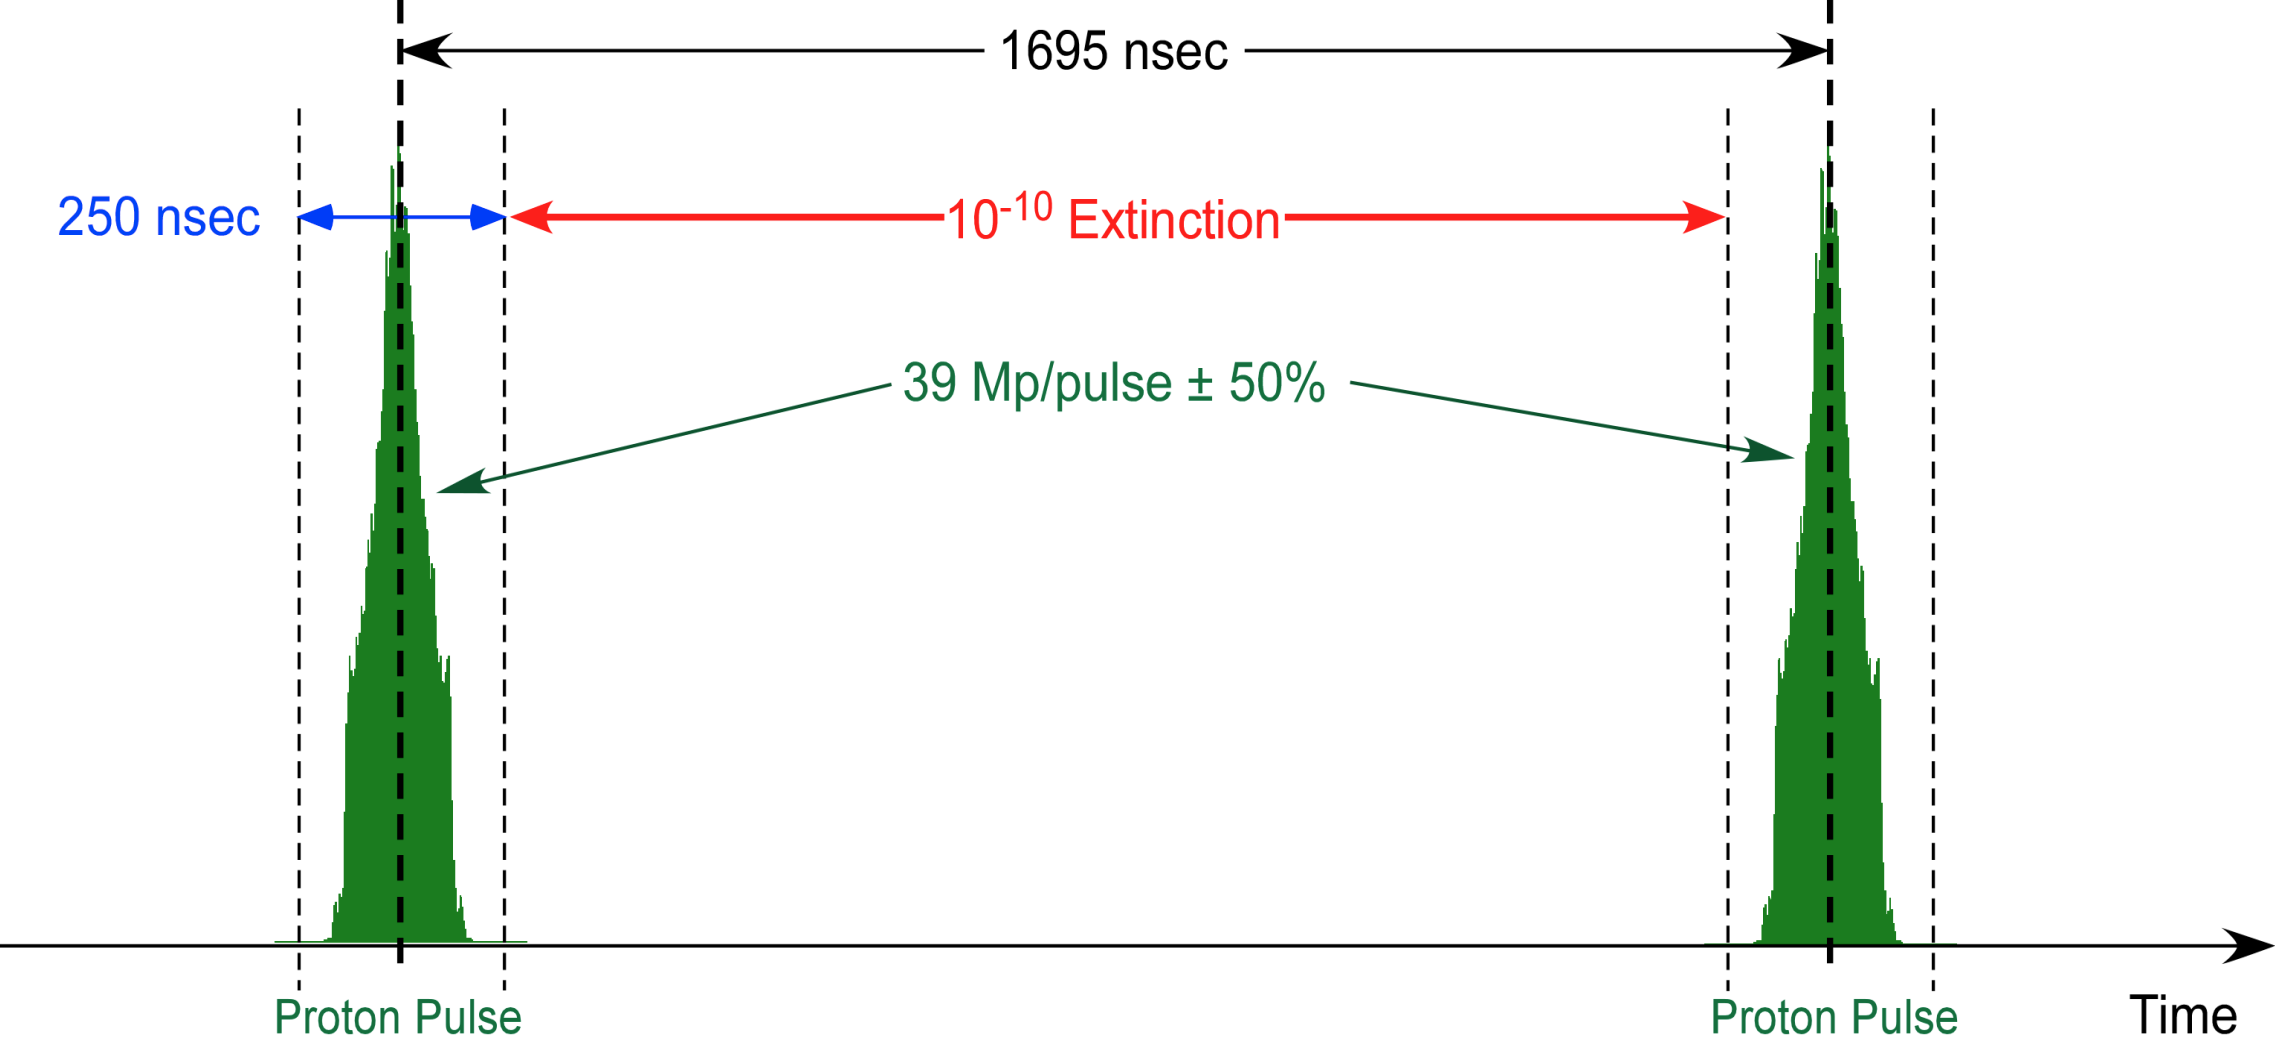
\includegraphics[width =\textwidth]{images/chapter2/Screenshot_20240301_151148.png}
\caption{Proton beam profile at the Mu2e Proton Target, Ref. \cite{accelerator}.}
\label{fig:beamprofile}
\end{figure}
Figure \ref{fig:beamprofile} illustrates the temporal profile of the beam at the Mu2e Proton Target. Consecutive proton pulses are spaced by 1695 ns. Each pulse lasts for 250 ns and contains $(3.9 \pm 2.0 )\times 10^7$ protons. The 1695 ns pulse separation is highly advantageous for the Mu2e experiment. Figure \ref{fig:beamwindow} shows the beam pulse, the simulated pion flux, the muon capture rate on the stopping target and the muon decay rate. The active window for detecting conversion electrons begins at $\sim$640 ns and extends for mor or less 1 $\mu$s. This selection finds a compromise between reducing pion-induced backgrounds  and increasing the rate of muon decays. Because of the brief lifetime of the pions, they are gone by the time the active window opens, resulting in a suppression of the pion count by $\mathcal{O}(10^{11})$. The 1695 ns pulse separation exceeds twice the muon lifetime, allowing sufficient temporal separation between prompt backgrounds and the live window without excessively compromising beam intensity.
\begin{figure}[!h]
\centering
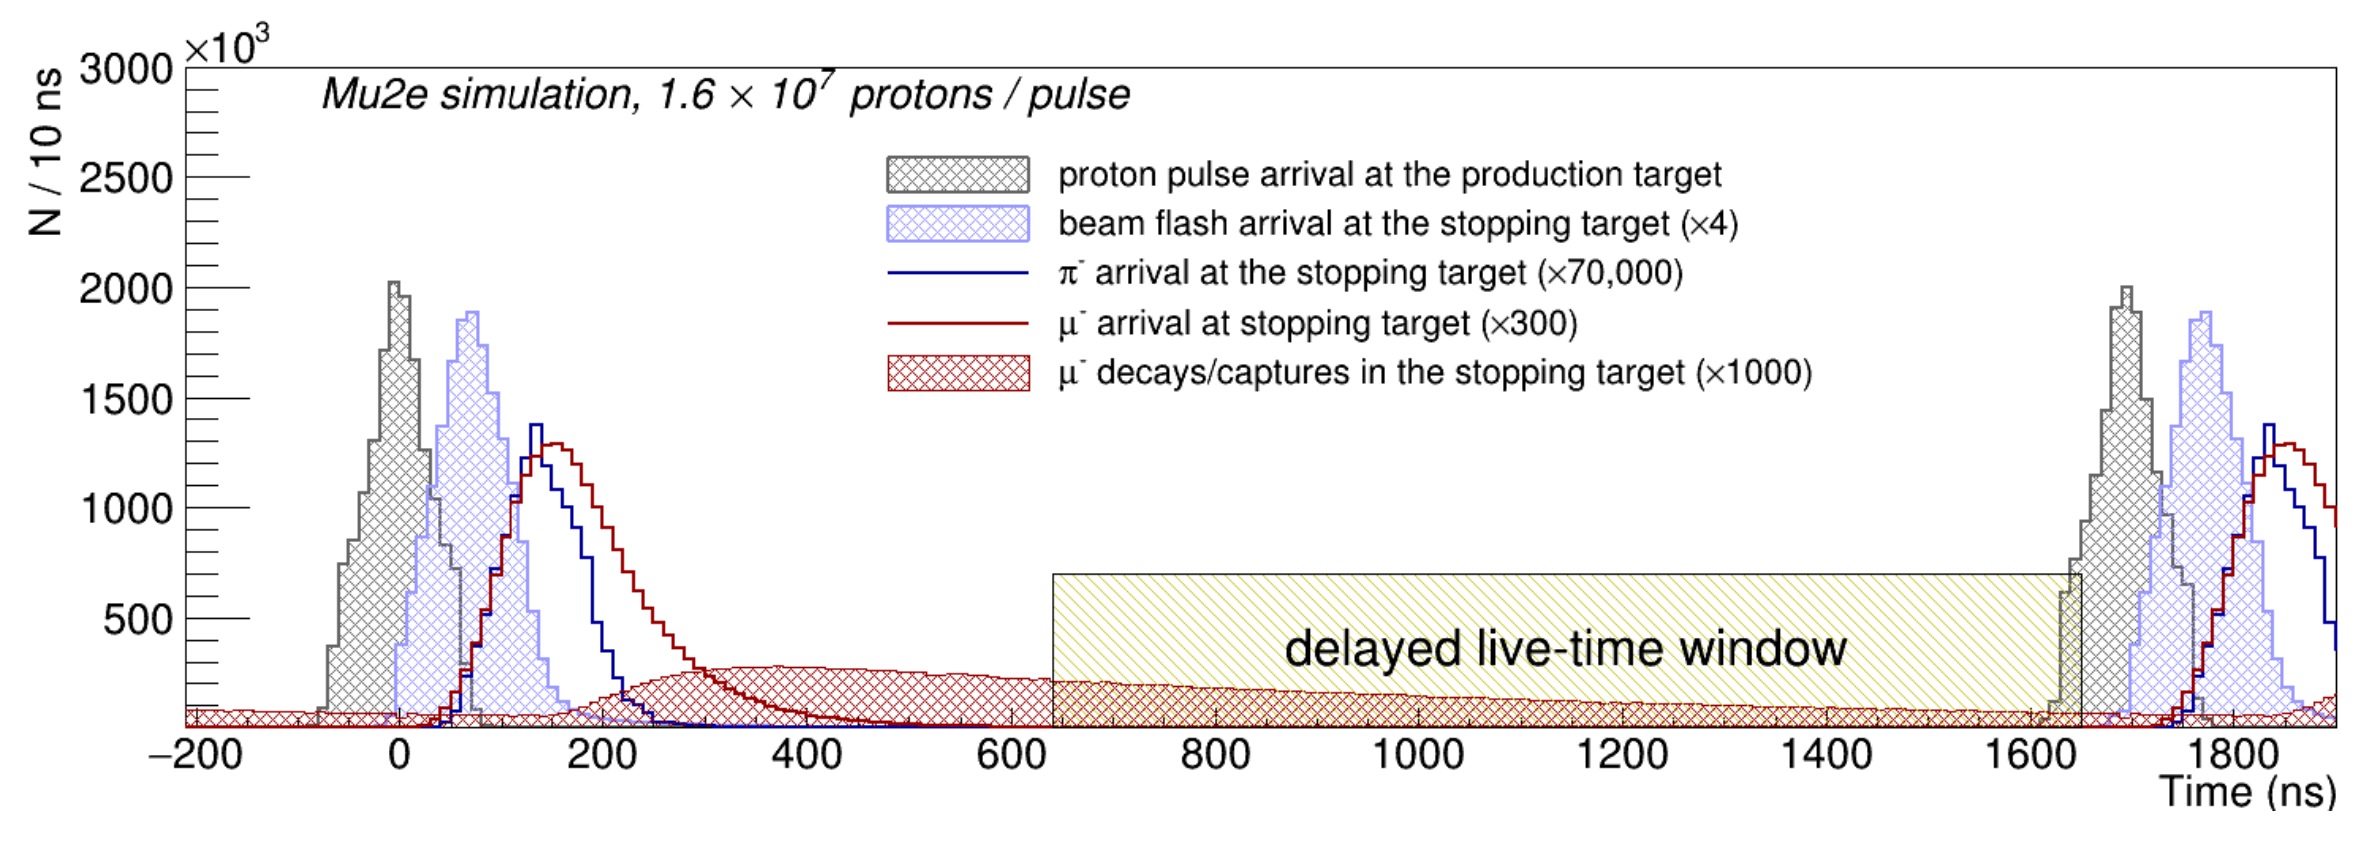
\includegraphics[width =\textwidth]{images/chapter2/Screenshot_20240301_164649.png}
\caption{Proton pulses arrive at the production solenoid every 1695 ns. A delayed live-time window can suppress the beam-related background, Ref. \cite{universe9010054}.}
\label{fig:beamwindow}
\end{figure}
\subsection{Proton Beam Extinction and Extinction Monitor}
As mentioned in the previous section, the Mu2e experiment requires the extinction level of the incoming proton beam, to reduce backgrounds caused by out-of-time protons. The extinction rate, defined as the ratio between the number of out-of-time protons and the number of the in-time protons, should be lower than $10^{-10}$, Ref. \cite{bartoszek2015mu2e}. The structure of the beam leads to an extinction level $2.1 \times 10^{-5}$. To take into account the fact that some beam will leak out of two consecutive proton pulses, an Extinction Insert is deployed in the M4 beamline between the Delivery Ring and the Mu2e experiment. The out-of-time beam particles are swept into a collimator system by a set of oscillating dipoles, called AC dipoles. These AC dipoles are simulated to offer an additional extinction factor of $5\times 10^{-8}$, reducing the overall extinction to $1.1 \times 10^{-12}$, leaving a margin of 10$^2$, Ref. \cite{accelerator}. An Extinction Monitor is positioned downstream of the production target along the proton beamline, Figure \ref{fig:extintion}. It monitors the extinction level of the incoming beam striking the Mu2e production target and delivers a measurement at a precision better than $10^{-10}$. The Extinction Monitor consists of a collimator and magnetic filter system, a pixel telescope, a system of trigger scintillators and a range-stack. The collimator and magnetic filtter system transport a small quantity of the particles generated at the production target to the Extinction Monitor. The pixel telescope tracks the trajectory of charged particles coming from the collimator. The pixel telescope consists of a permanent magnet and 8 scintillators, as shown in Figure \ref{fig:extintionmonitor}. The system uses a permanent magnet to separate two sets of four scintillator planes, allowing for momentum measurements of entering particles. The range stack is located further downstream from the pixel telescope. Steel absorber plates separate scintillators, distinguishing between hadrons and muons based on their penetrating capacities.
\begin{figure}[!h]
\centering
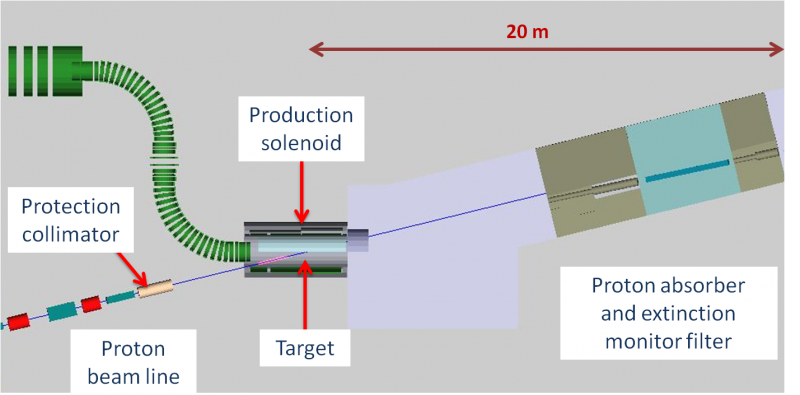
\includegraphics[width =\textwidth]{images/chapter2/800px-Extinction_filter.png}
\caption{The Extinction Monitor is located downstream of the
production target, Ref. \cite{Prebys:IPAC2015-THPF121}.}
\label{fig:extintion}
\end{figure}
\begin{figure}[!h]
\centering
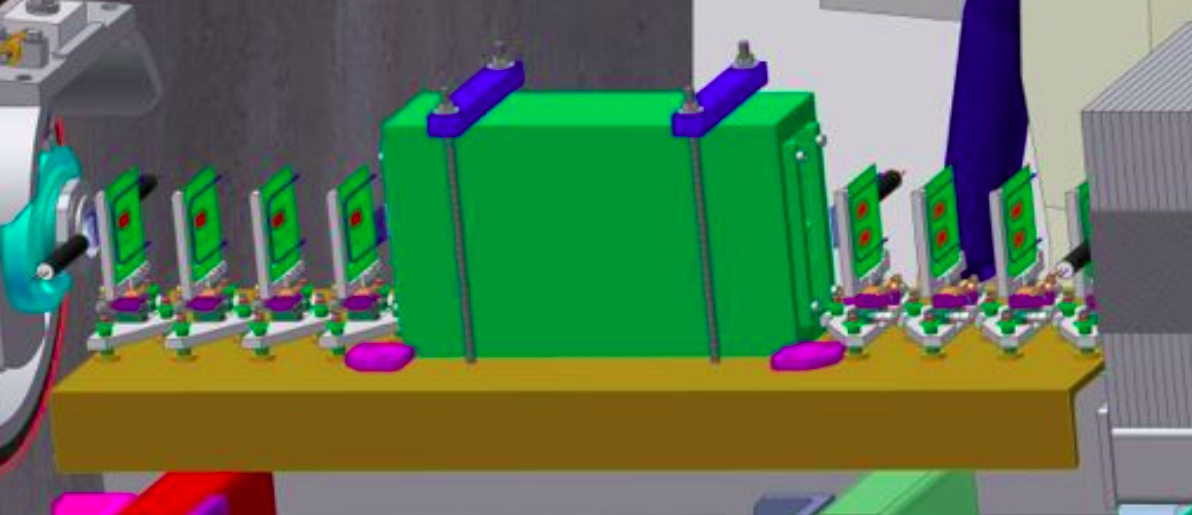
\includegraphics[width =0.9\textwidth]{images/chapter2/Screenshot_20240306_184720.png}
\caption{The tracking spectrometer of the Mu2e experiment, consisting of eight planes of pixel detectors and a permanent magnet spectrometer, Ref. \cite{Prebys:IPAC2015-THPF121}.}
\label{fig:extintionmonitor}
\end{figure}
\subsection{Production Target}
The Mu2e production target is an additional essential element of the accelerator systems. It is suspended in the middle of the PS bore, Ref. \cite{bartoszek2015mu2e}. It is made of tungsten. The tungsten has a high pion production cross-section, capable of producing the necessary number of stopped muons. The refractory material allows the target to be cooled radiatively without the need of any extra cooling equipment. A compact design minimizes pion reabsorption on the production target.
\section{Solenoids System}
The Mu2e Solenoid system consists of three magnetically coupled systems: the \textbf{Production Solenoid} (PS), the \textbf{Transport Solenoid} (TS) and the \textbf{Detector Solenoid} (DS), shown in Figure \ref{fig:mu2escheme}. Each system contains multiple module and each one is made of superconducting coils wound with aluminum stabilized Nb-Ti Rutherford cables, located in a 4.5 m long cryostat. The shape of solenoids is designed in order to efficiently transmit muons and to suppress other particles. The resulting magnetic field is $\mathcal{O}$(1 T): its highest value is 4.6 T at the upstream end of the experiment and the lowest value is 1 T at the downstream end. The muons are guided toward the stopping target and the DS by lowering the magnetic field. Local magnetic field minima are avoided to avoid trapping particles in these areas. In the PS, the magnetic field decreases from 4.6 T to 2.5 T at the entrance of the TS. The large gradient helps to collect the secondary pions and muons and to direct them towards the DS. The magnetic field across the S-shaped TS changes its value only by a factor of 0.5 T. The shape of the TS allows to not transmit photons and other neutral particles in the DS and its dimension was set to avoid transmitting particles with large momentum. These particles either spiral with a large helical radius (large initial momenta perpendicular to the field) or cannot create an S-shaped bend (large initial momenta parallel to the magnetic field), resulting in collisions with solenoid walls or collimators. As particle drifts in the solenoid field is dependent on the particle charge, positively and negatively charged muons drift in opposite vertical directions and are separated, as explained in Appendix \ref{appendix1}. In the upstream curved solenoid portion, as shown in Figure \ref{fig:collimators}, the spiraling positive (blue) and negative (red) muons are deflected downwards and upwards respectively. Positive muons are stopped in collimators COL3u and COL3d. The TS is long enough for pion decay, suppressing RPC backgrounds. It also protects the detectors from radioactively hot areas around the primary beam and the production target. The magnetic field in the first half of the DS is reduced from 2 T to 1 T. In a smoothly gradient field, the adiabatic invariance of the magnetic flux can be used. Assuming a constant $p^2_\perp/B$, there is:
\begin{equation}
    v^2_{\parallel}=v^2_0-v^2_{\perp 0}\frac{B(z)}{B_0}
\end{equation}
Here, $\perp$ is referred with respect to the magnetic field $B$ and $\parallel$ is referred to the $z$ direction. The subscript 0’s indicates the initial state. The gradient pitches electrons forward into the tracker's acceptance while rejecting higher velocity electron, as mentioned in \ref{beamelectrons}. 
The second half of the DS containing the Tracker and the Calorimeter has a uniform magnetic field of 1 T. This allows particle trajectories and momenta to be reliably measured.
\begin{figure}[!h]
\centering
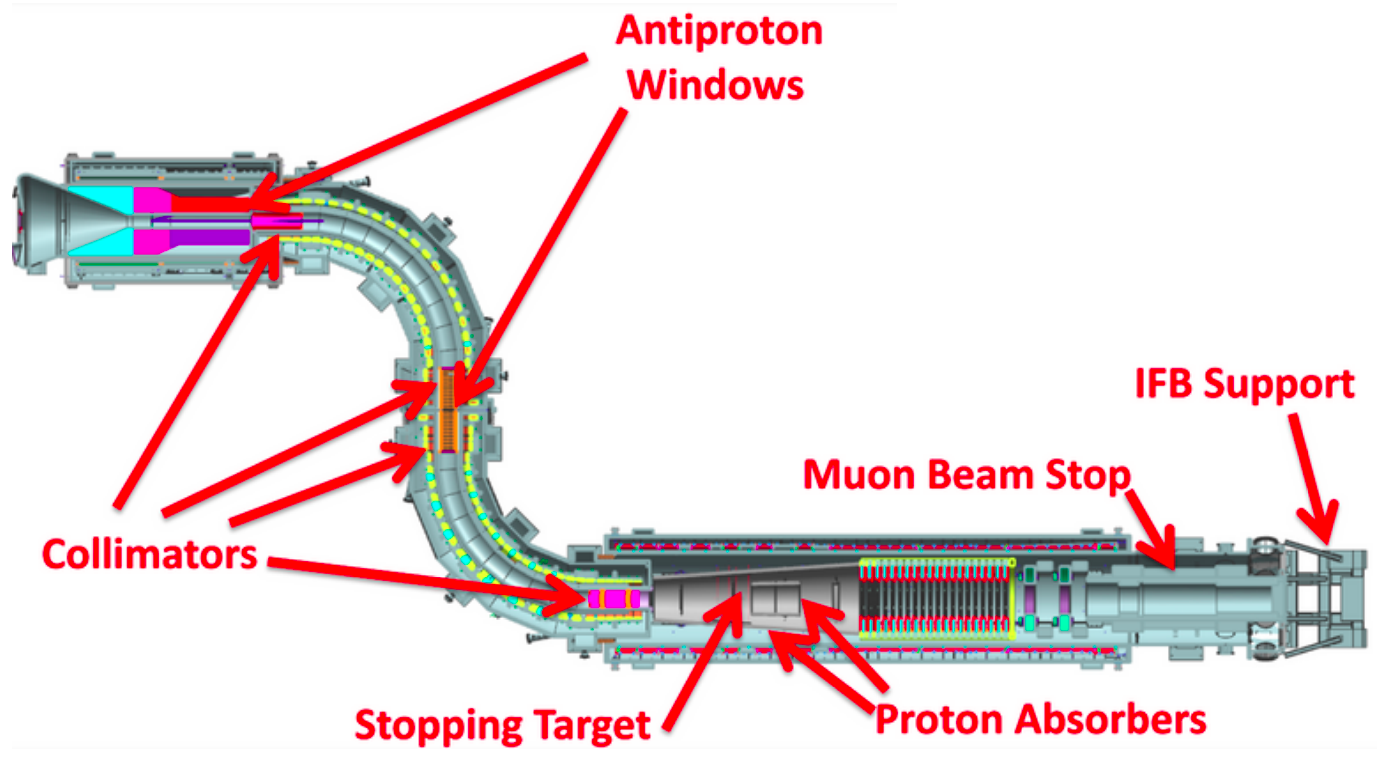
\includegraphics[width =0.9\textwidth]{images/chapter2/Screenshot_20240303_152845.png}
\caption{The muon beamline, composed of the Production Solenoid (PS), the Transport Solenoid (TS) and the Dector Solenoids (DS), Ref. \cite{ginther}. The PS is 4 m long. The role of the PS, shown in Figure \ref{fig:PS}, is to collect pions, kaons and their decay products muons. The TS is S-shaped and it is divided in five parts. The first is called TS1 that contains the first collimator (COL1), made of copper wedges. It filters particles from their momentum and reduces the radiation damage for coils of the upstream part of the TS (TSu). The TS2 contains a toroidal field in order to select negative muons from the positive ones in TS3 with two rotatable collimators (COLu and COLd). The rotatable feature allows selection of $\mu^-$'s instead of $\mu^+$'s, which can be used for detector calibration. The TS4 role is to put the beam in the center of the solenoid. TS5 connects TS with DS and it contains a collimator (COL5) made of polyethylene, which will serve as a shield from neutrons. A thin window assembly is installed at the beginning of the TS and also between the rotatable collimators to absorb antiprotons in the beam.
The DS, shown in Figure \ref{fig:DS}, is a cylindrical system of approximately 11 m in length and 2 m in radius, which houses the Stopping Target and the main Mu2e detectors. The system is divided into two sections: a 4 m gradient section following the TS and a 6 m spectrometer section. The gradient region allows to separate conversion electrons from beam electrons. In the spectrometer region, the uniform magnetic field allows a precise measurement of the particle momentum. The upstream part of the beamline accounts for the Production Solenoid (PS) and the first part of the Transport Solenoid (TSu). The downstream part is composed of the last portion of the Transport Solenoids (TSd) and the Detector Solenoid (DS). Protons from muon captures in the Stopping Target are partially suppressed by a 0.5 mm thick cylindrical-shaped polyethylene proton absorber, placed halfway between the Stopping Target and the tracker. Finally, the IFB is a plate at the end of the DS, maintaining the DS vacuum and providing a path for the services and signals between vacuum and hall air.
}
\label{fig:muonbeamline}
\end{figure}
\begin{figure}[!h]
\centering
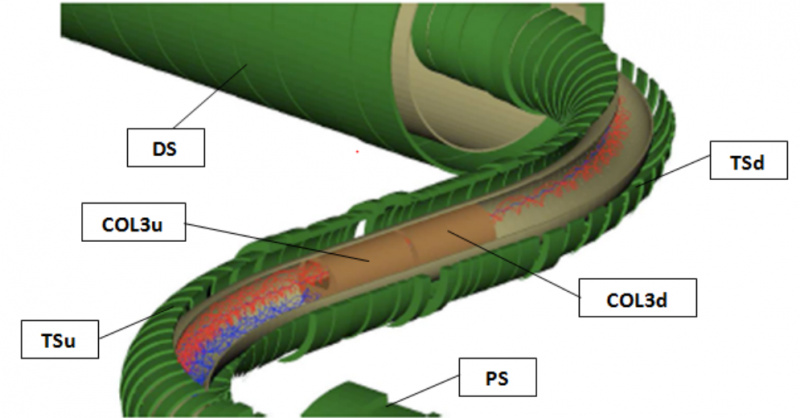
\includegraphics[width =0.95\textwidth]{images/chapter2/800px-MuonBeamlineCollimators2.png}
\caption{The view of the Transport Solenoids and the collimators COL3u and COL3d showing the offset apertures in those collimators. The upper spiraling negative muons (red) pass through the aperture while the positive muons (blue) are stopped by these collimators, Ref. \cite{tsview}.}
\label{fig:collimators}
\end{figure}
\begin{figure}[!h]
\centering
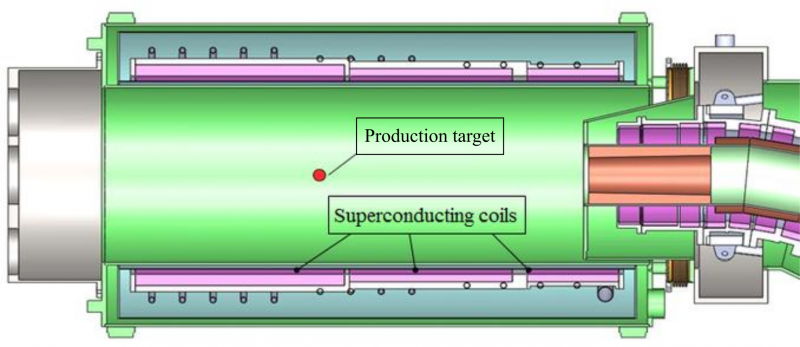
\includegraphics[width =0.95\textwidth]{images/chapter2/800px-Production_solenoid.png}
\caption{Cross-section of the production solenoid, Ref. \cite{6376120}.
The production target is placed approximately at the center of the superconducting coils.}
\label{fig:PS}
\end{figure}
\begin{figure}[!h]
\centering
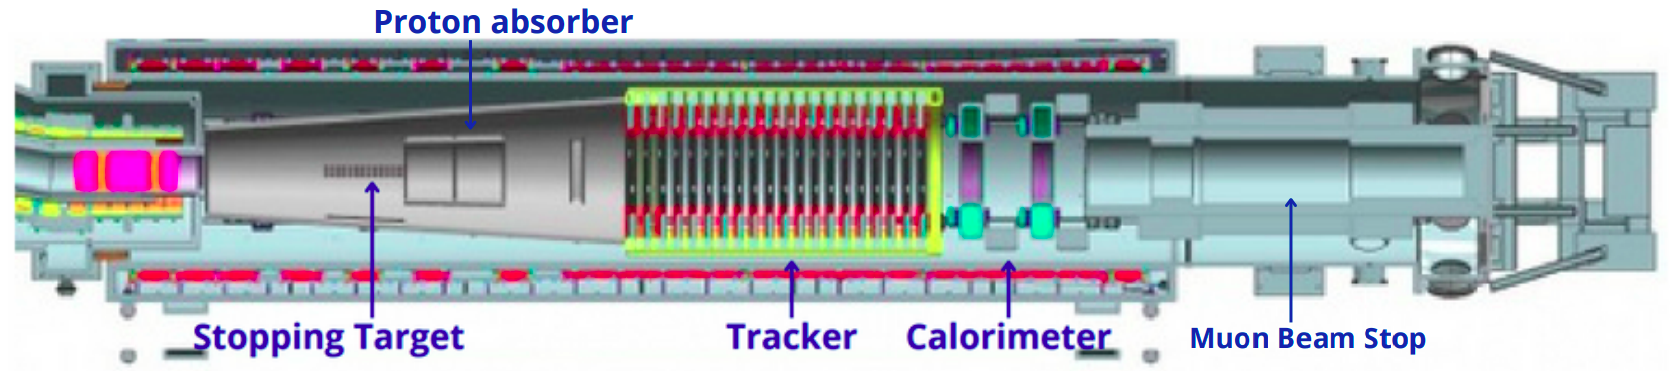
\includegraphics[width =0.95\textwidth]{images/chapter2/Screenshot_20240306_225639.png}
\caption{Overall structure of the Detector Solenoid coils and cryostat, Ref. \cite{bobbb}.}
\label{fig:DS}
\end{figure}
\section{Stopping target}
The Mu2e muon stopping target is composed of 37 annular aluminum foils  with a purity of above 99.99\%, Ref. \cite{bobbb}. The foils are 100 $\mu$m thick, minimizing energy losses of the conversion electrons. This design narrows the reconstructed conversion electron momentum distribution and separates it from the DIO electron momentum distribution. The annular design reduces interactions with the beam electrons and other particle released in muon nuclear captures, which can create particle sprays and damage to the tracker's internal components. The central hole does not affect the target capacity to halt muons, which move in helical patterns. Muons passing through the hole of an upstream foil will stop in a downstream layer. There are various factors to consider while selecting aluminum as the stopping target material. First, as described in Section \ref{backgrounds}, the aluminum target has a low RMC background. Moreover, the muonic aluminium atom has a quite long lifetime, as shown in Figure \ref{fig:muonicatom}. The long lifetime allows separation between prompt backgrounds and a live window with a good decay rate. The muon DIO endpoint energy, further, depends on the type of nucleus, as shown in Figure \ref{fig:endpoint}. Aluminum has a high endpoint energy, so when muons are captured on other detector materials with a higher atomic number $Z$, they have lower endpoint energies and do not contribute to background. Aluminum is a suitable stopping target material for muon-to-electron conversion searches.
Moreover, the branching ratio ($BR$) of the conversion varies depending on the stopping target material due to differences in atomic number ($Z$) and mass number ($A$). By comparing $BR$s on different nuclei normalized to aluminum, it's possible to identify the dominating operator type, such as scalar ($S$), dipole ($D$), vector of transition charge radius type and vector of effective $Z$-penguin type, ($V(\gamma)$) and ($V(Z)$) respectively. Despite challenges in separating prompt backgrounds from signals due to short lifetimes of muonic atoms, materials with higher $Z$ offer better model differentiation. If the Mu2e experiment observes conversion signals, a subsequent search, Mu2e-II, could employ titanium as the stopping target. A more detailed discussion can be found in Ref. \cite{PhysRevD.80.013002}, \cite{PhysRevD.76.059902} and \cite{abusalma2018expression}.
\begin{figure}[!h]
\centering
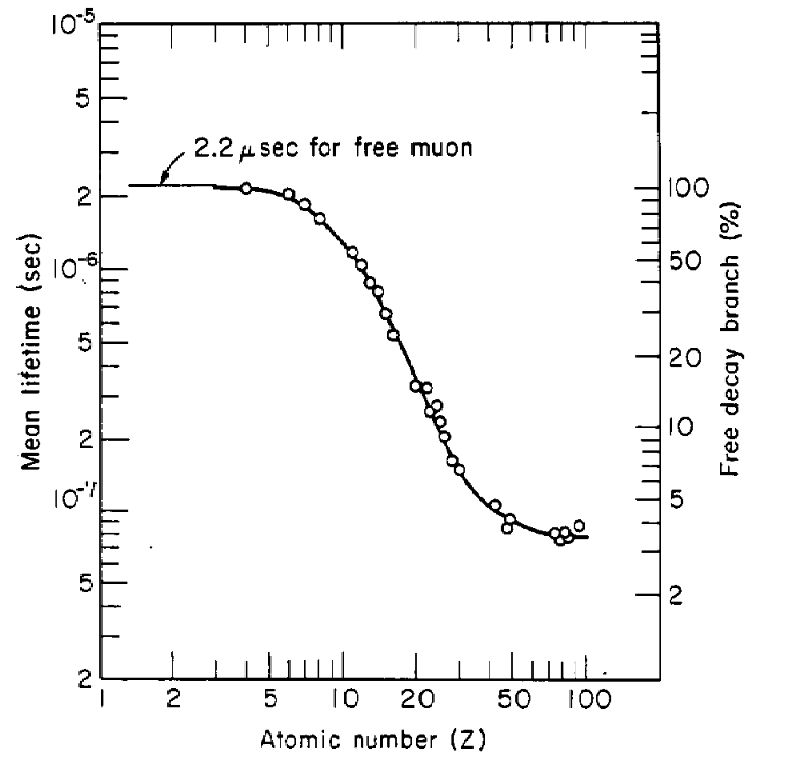
\includegraphics[width =0.5\textwidth]{images/chapter2/lifetime_mu_matter.png}
\caption{ The mean lifetimes and free decay branches of the muonic $1s$ state versus the atomic number of the nucleus to which the negative muon is bound \cite{TYamazaki_1975}.}
\label{fig:muonicatom}
\end{figure}
\begin{figure}[!h]
\centering
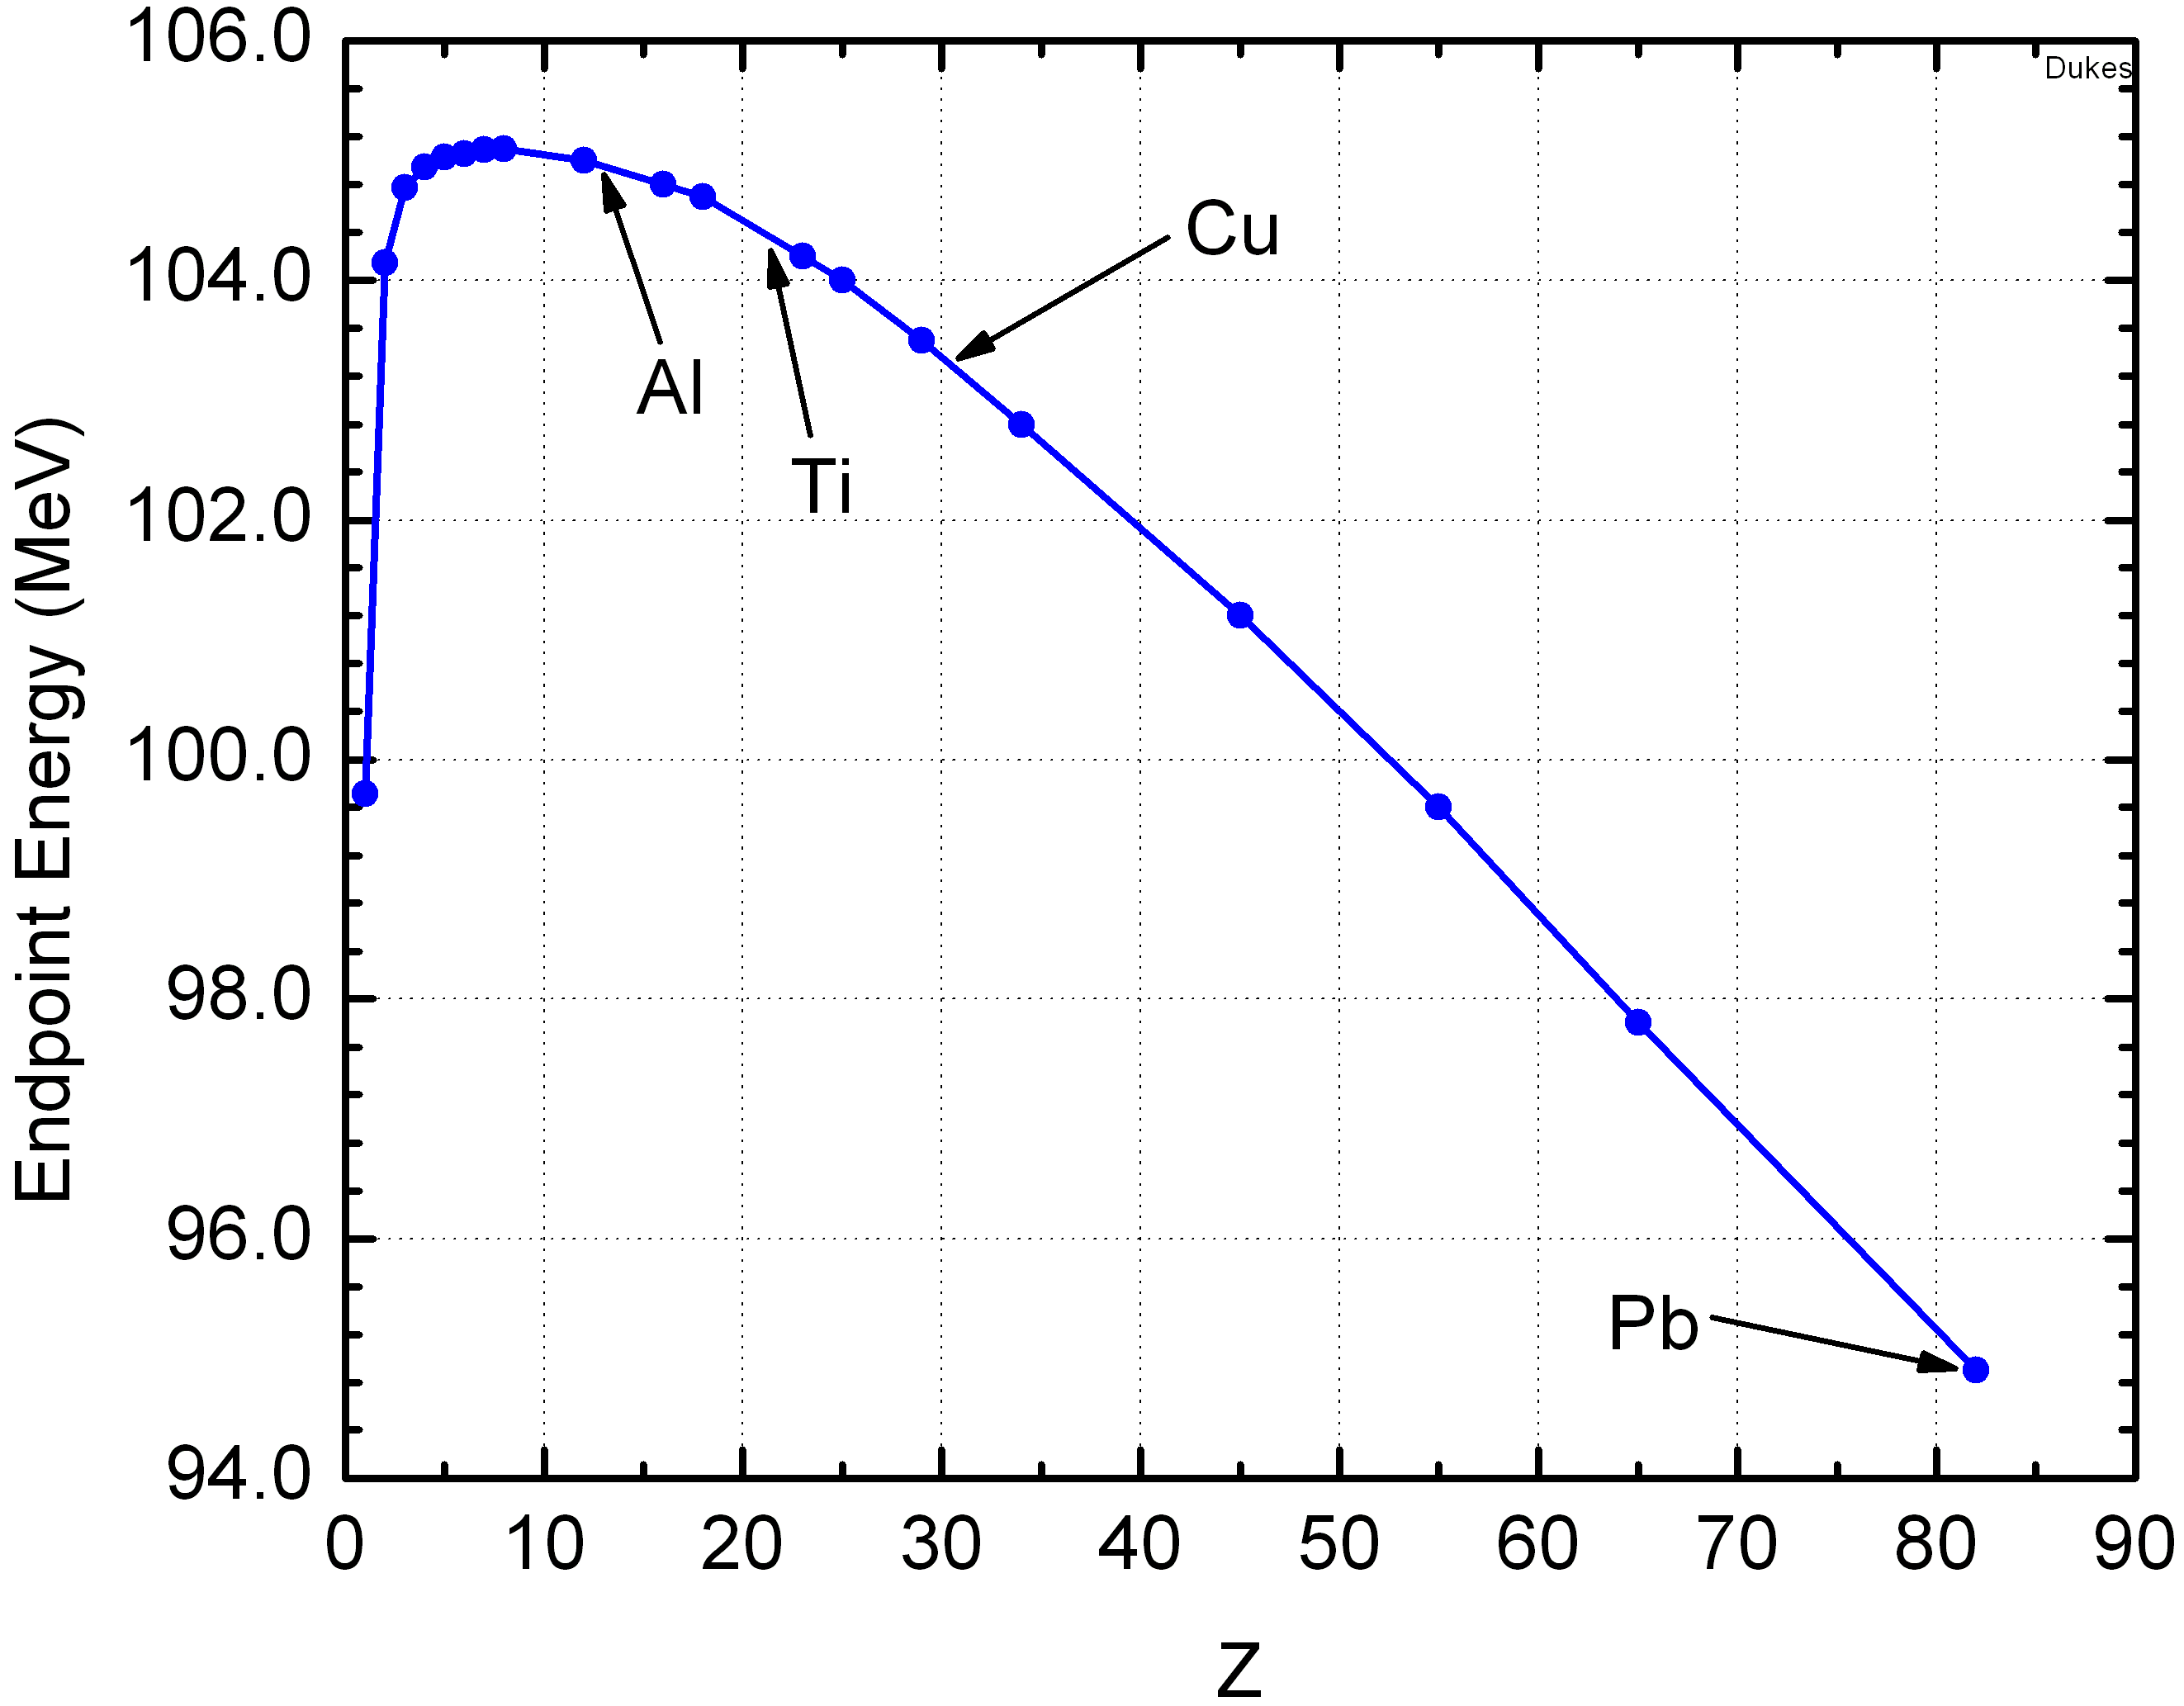
\includegraphics[width =0.5\textwidth]{images/chapter2/endopint.png}
\caption{ The dependence of electron energy spectrum endpoint from muon DIO, Ref. \cite{dukes}.}
\label{fig:endpoint}
\end{figure}


\section{Detectors}
\subsection{The Tracker}\label{trackersec}
The Mu2e Straw Tube Tracker will measure conversion electrons momentum. It is located inside the DS, downstream of the stopping target. Its shape follows the helical trajectories of conversion electrons in the magnetic field. The Mu2e Tracker detects particles using gas drift tubes, \textit{straw tubes}. 96 straw tubes are arranged in two staggered layers to form a panel, Ref. \cite{bartoszek2015mu2e}. This is the basic standalone module both mechanically and electrically, as shown in Figure \ref{fig:trkpanel}, upper left. Each panel, that is harp-shaped, spans 120°. The straw tubes are arranged like harp chords. The electronics is stored in the outer volume. The Mu2e Tracker has a very limited material component, particularly in the straw region, which reduces the probability of scattering conversion electrons and increases the momentum resolution. The panels are combined using the approach indicated in Figure \ref{fig:trkpanel}, upper right, Ref. \cite{trk}. Three panels create a full circle and two layers of six panels, rotated by 30°, form a plane. A station is made up of two planes that have been rotated by 60°. One or more panels cover the entire annular region. The entire Tracker consists of 18 identical stations, shown in Figure \ref{fig:trkpanel}, bottom. It is 3.2 metres long and 1.7 metres in diameter. 
\begin{figure}[!h]
\centering
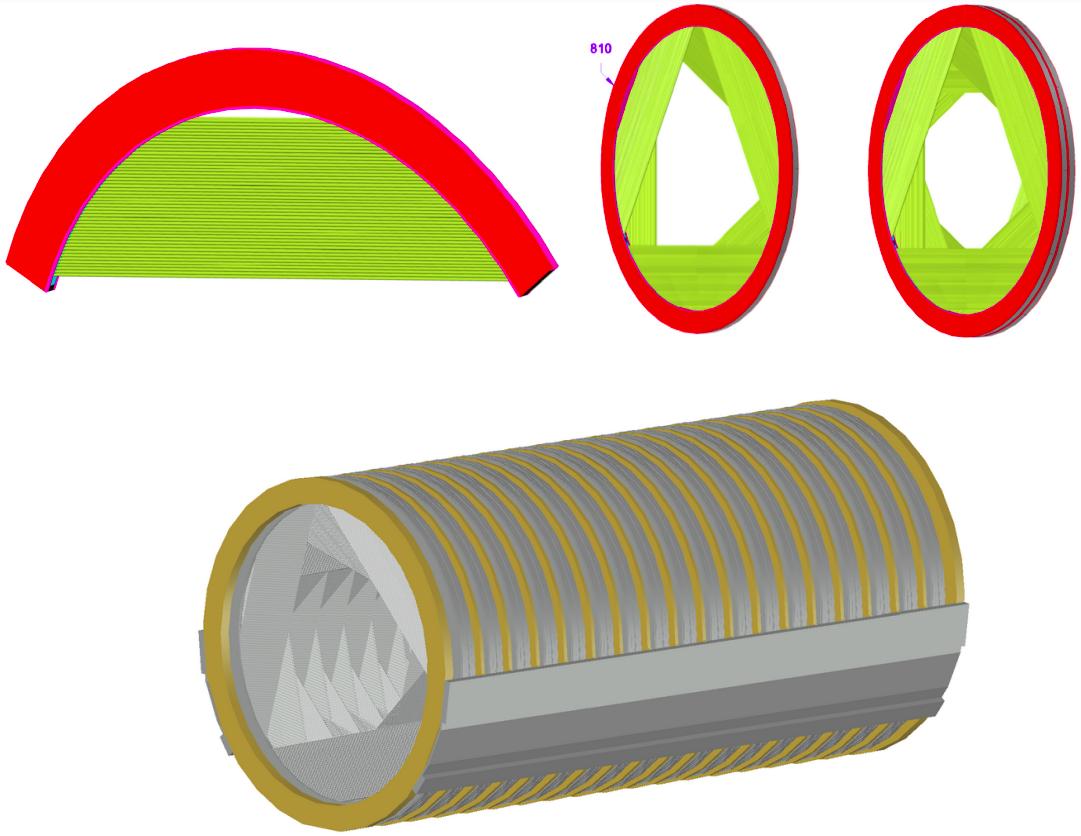
\includegraphics[width =0.7\textwidth]{images/chapter2/Screenshot_20240306_222803.png}
\caption{(Upper left) Tracker panel. (Upper right) Isometric view of a tracker plane (left) with three panels each on the front and back face and a station (right) consisting of two planes. (Bottom) The assembled tracker, with 18 stations. Stations are shown in grey and support structure in gold, Ref. \cite{bartoszek2015mu2e}.}
\label{fig:trkpanel}
\end{figure}
Figure \ref{fig:sttrk} shows that the Tracker straws are only in the active region with radius r ranging from 380 mm to 700 mm. The central part of the Tracker is not instrumented. A similar annular design can also be found in the Mu2e Calorimeter, in Section \ref{calorimeter}. The geometry of the detector is specifically designed to reduce background. Detectors are blind to muon beams and associated activity, including $\pi$-DIF, $\mu$-DIF, beam electrons and other particles emitted during nuclear captures. his shape prevents the detection of low-energy electrons released during muon DIO. Figure \ref{fig:sttrk} shows the electrons trajectory as coloured circles passing through the stopping target. For a homogeneous magnetic field, the radius of a helix follows the equation \ref{partincamp}, so it is proportional to transverse momentum of the particle. Low momentum electrons, $\lesssim$ 53 MeV/c, can pass through detectors without causing a hit. This corresponds to the green trajectory in Figure \ref{fig:sttrk}, whereas the green circle represents an example trajectory. Electrons with higher momenta can leave some hits on the detectors, but few hits are insufficient to reconstruct the electron trajectory, orange trajectory shown in Figure \ref{fig:sttrk}. The tracks are only reconstructible when the electron momentum is high enough: $\gtrsim$ 90 MeV/c. It is expected that only muon DIO events will be recorded in the Tracker. The low rate simplifies front-end electronics (FEE) requirements and minimises reconstruction mistakes caused by accidental activity. Chapter \ref{chaptertrk} will provide a detailed discussion of the straw tube Tracker panel, including its detection mechanism, mechanical design, front-end electronics and data acquisition (DAQ) system, as the focus of my thesis is on the Vertical Slice Test of the straw tracker.
\begin{figure}[!h]
\centering
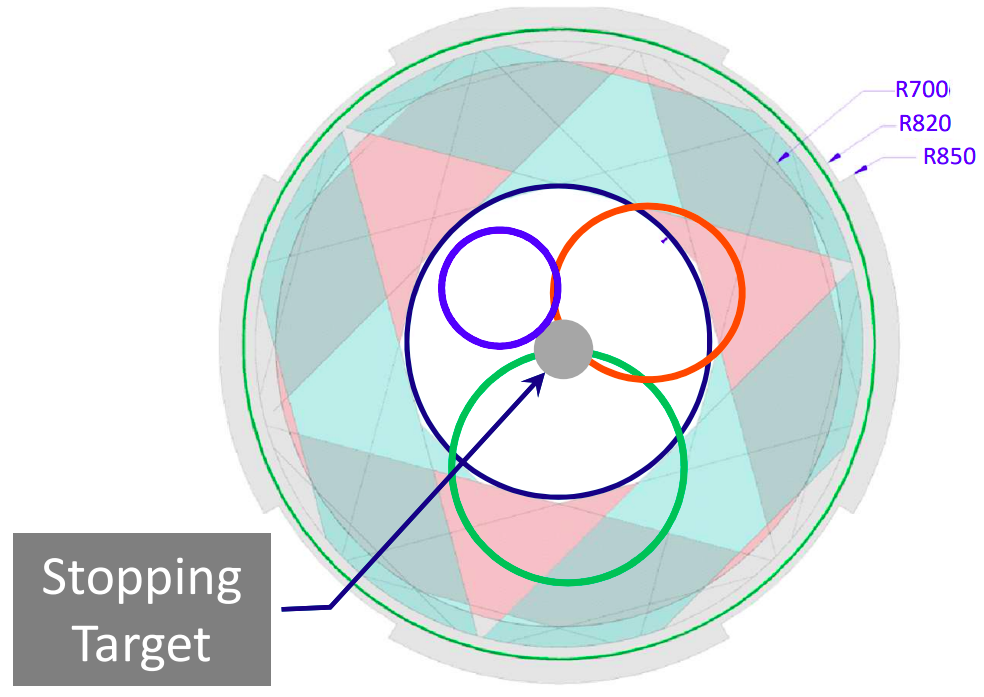
\includegraphics[width =0.7\textwidth]{images/chapter2/Screenshot_20240306_214911.png}
\caption{The annular design of Mu2e detectors: a view of the Tracker, Ref. \cite{trk}.}
\label{fig:sttrk}
\end{figure}
\subsection{The Electromagnetic Calorimeter}\label{calorimeter}
\subsection{Cosmic Ray Veto}\label{CRV}
As stated in Section \ref{backgrounds}, Mu2e expects backgrounds generated by cosmic rays at a rate of one per day. Although the EM Calorimeter can detect some backgrounds created by muons with the correct momenta, there are still problematic cases. To reduce these backgrounds, Mu2e employs an active veto system combined with shielding. An overview of the Cosmic Ray Veto (CRV) is shown in Figure \ref{fig:crv}. It covers the entire DS and half of the TS (there is no veto at the bottom), for a total area of 327 m$^2$.
The CRV modules are manufactured from plastic scintillator extrusions. Each extrusion has a cross-sectional area of $5 \times 2$ cm$^2$, with different lengths. The extrusions are coated with titanium dioxide to improve internal reflections and so the light yield. Two grooves are extruded inside the scintillator bar throughout its length, containing 1.4 mm diameter wavelength changing fibres. They send light to the extrusion ends, where each fibre is detected by a $2 \times 2$ mm$^2$ SiPM on each end. Figure \ref{fig:crvmodule} illustrates the cross-section of the CRV module. Each module has four overlapping layers of plastic scintillator counters to reduce the effect of gaps. The layers are separated by $\sim$ 10 mm aluminium plates used as absorbers. When three of the four layers of the CRV are activated, a veto window of $\pm$125 ns is provided. A conversion-like signal observed during this time window is assumed to be produced by a cosmic-ray muon. The anticipated total dead time is $\sim$5\%. The CRV system should be highly efficient. The success of the experiment depends on a detection effectiveness of 99.99\% or higher.

\begin{figure}[!h]
\centering
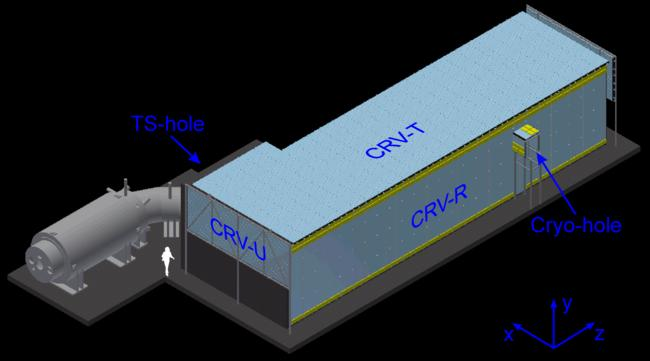
\includegraphics[width =0.85\textwidth]{images/chapter2/Crv_downstream.jpg}
\caption{The cosmic ray veto covering the Detector Solenoid looking upstream, showing the downstream (CRV-D), left (CRV-L), top (CRV-T) sectors, as well as the hole where the transport solenoid enters the enclosure, Ref. \cite{bartoszek2015mu2e}.}
\label{fig:crv}
\end{figure}

\begin{figure}[!h]
\centering
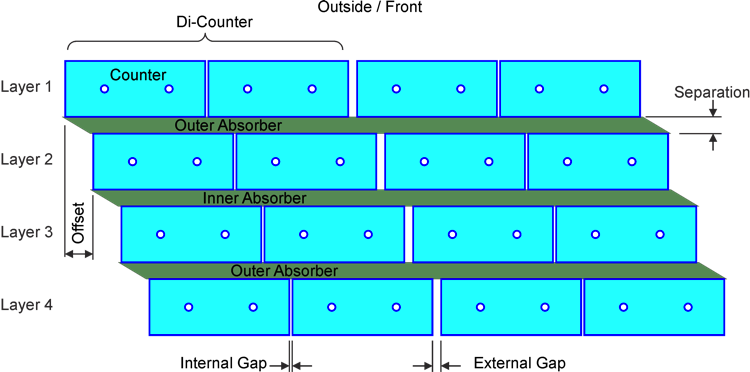
\includegraphics[width =0.85\textwidth]{images/chapter2/Crv_module_geometry.png}
\caption{The CRV module geometry and nomenclature. Internal gaps are those between the counters in a di-counter, Ref. \cite{Giovannella_2020}.}
\label{fig:crvmodule}
\end{figure}
\subsection{Stopping Target Monitor}
A Muon Beam Stop (MBS) is installed at the downstream end of the DS to absorb muons that are not stopped in the stopping target, Ref. \cite{bartoszek2015mu2e}. The MBS is intended to limit the effects of muon decay and capture inside the stop. The magnetic field gradient prevents the majority of the low-energy charged particles created in the MBS from moving upstream. It is made from high-$Z$ minerals and polyethylene. Muons have an extremely short lifetime in high-$Z$ materials, as shown in Figure \ref{fig:muonicatom}, enabling activities to take place before the live window starting at 640 ns. Polyethylene, on the other hand, absorbs protons and neutrons emitted by excited nuclei created during muon capture.
The Stopping Target Monitor, STM, is placed downstream of the MBS to measure the number of muons collected on the stopping target, because of the extremely high x-ray and gamma rates, as shown in Figure \ref{fig:stm}. This number will be used as denominator in $R_{\mu e}$. Mu2e detects the x-ray spectrum released when muons are stopped on a stopping target and fall to the ground state. The experiment uses 357 keV x-ray photons created when muons go from the $2p \rightarrow 1s$ state, Ref. \cite{bobbb}, and aims to measure the number of stopped muons with the 10\% of accuracy. The STM employs an x-ray detection device, a high purity germanium (HPGe) solid-state detector. The detector should only view the target, if possible. A requirement is a good collimation ahead of the detector. It sees the stopping target through a stainless steel pipe 10 cm in diameter and 3 m long, tunneling through the MBS near the DS axis, Ref. \cite{stm}. Collimators inside the pipe give the STM a clear view of the stopping target while obscuring other components, such as the downstream collimator in the TS. HPGe devices are too slow to track individual occurrences. In addition, the germanium lattice is sensitive to radiation damage. To keep radiation damage and rates under control, the STM is approximately 35 m from the stopping target and is well-insulated. An alternative method measures the delayed photons released during the beta decay of $^{27}$Mg, which occurs in 13\% of muon catches. The excited $^{27}$Mg decays to an excited state of $^{27}$Al with a half-life of 9.5 min, emitting an 844 keV photon within ps that can be detected. This method uses the pulsed beam macrostructure (the 1.4 s cycle) to detect only proton batches that are not transmitted to Mu2e.
\begin{figure}[!h]
\centering
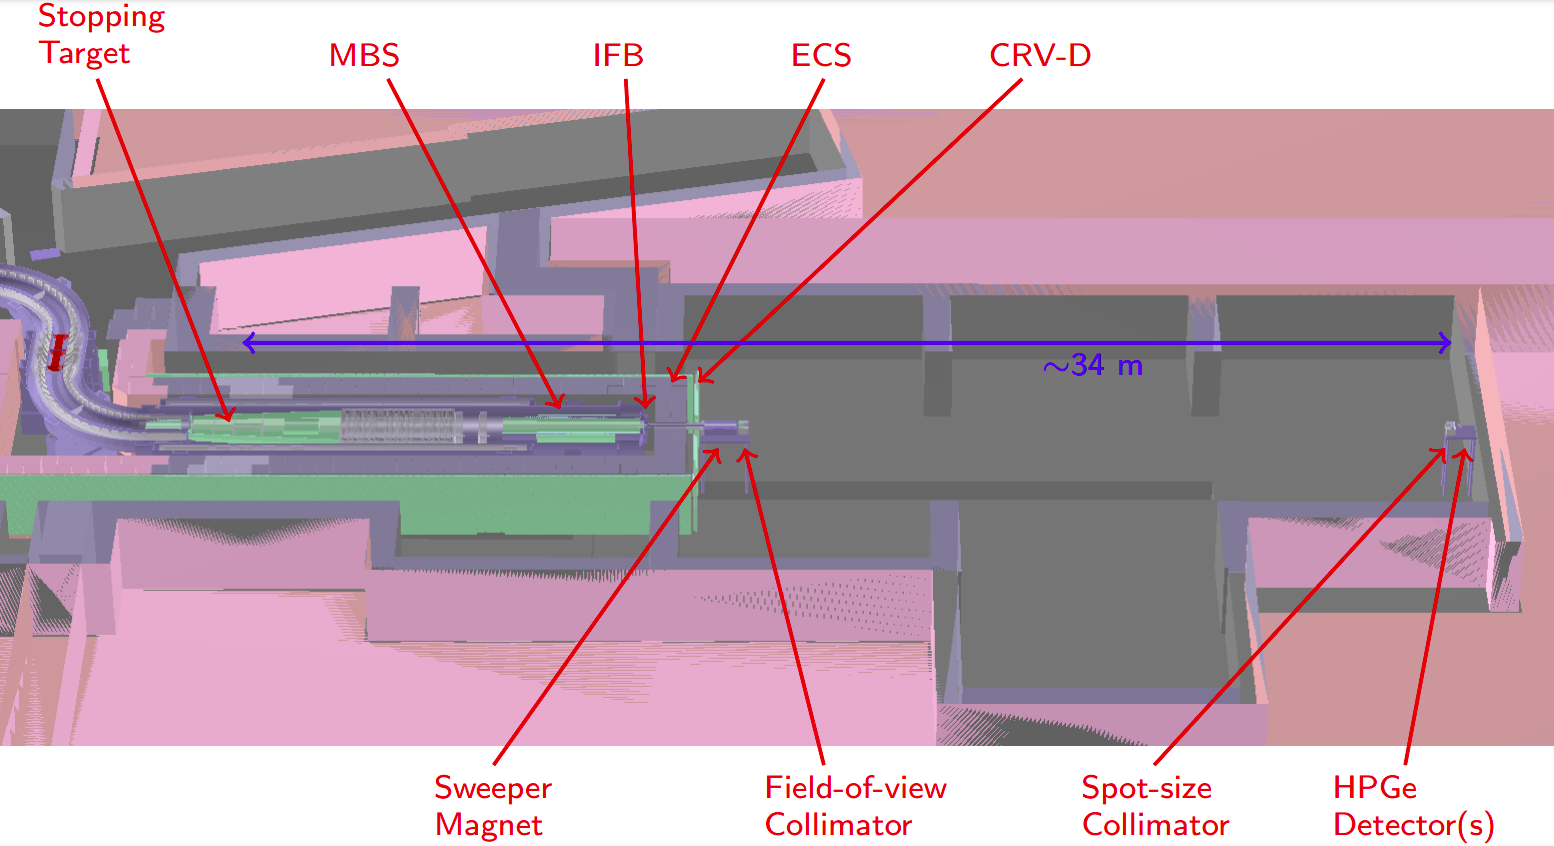
\includegraphics[width =\textwidth]{images/chapter2/Screenshot_20240306_180910.png}
\caption{The Stopping-Target Monitor geometry showing the DS region (left), the End Cap Shielding, sweeper magnet and STM field-of-view collimator. At the far end of the hall (right) is the final $spot-size$ collimator and the STM detector.}
\label{fig:stm}
\end{figure}
\section{Firmware-Based Data Acquisition}
The Mu2e Trigger and Data Acquisition (TDAQ) system collects digitized data from the Tracker, Calorimeter, Cosmic Ray Veto and Beam Monitoring components (Stopping Target Monitor and Extinction Monitor) and delivers that data to online and offline processing for analysis. It must merge data from $\sim$450 subsystems and apply filters to reduce data volume by a factor of 100 before storing it offline. It is also responsible for detector synchronization, control, monitoring and operator interfaces. The Mu2e DAQ system uses a $streaming$ readout technique, which means that all detector data from the experiment is digitized and zero-suppressed in their respective Front End Electronics (FEEs) before being transferred. This strategy results in a high data flow in the DAQ system while providing greater flexibility in data selection and analysis.
\subsection{Expected rate}
The data-taking periods will be divided in two modes: on-spill and off-spill. The on-spill mode covers periods when 8 GeV proton bunch are colliding the production target. The off-spill mode covers all other periods: between bunches, calibration periods, commissioning. 
Calling what is written in section XX, it is possible to estimate the on-spill event contribution:
\begin{itemize}
    \item 43.1ms (time of one spill)/ 1695ns(digitization time) = 25K pulses per spill
    \item 8(number of spills)*25K=200K on spill events /cycle
    \item 200K/ 1.4s(cycle time) = 145K ON Spill events/s
\end{itemize}
di questi 1.4s, 1.055s si riferisce all'offspill e 0.4s all'onspill.
Meanwhile, the off-spill event contribution is:
\begin{itemize}
    \item 145K ON Spill events/s*0.4s=58Kevents
    \item 55 K /1.4s= 41K off spill events per second per cycle
\end{itemize}
buffering: 0.4/1.4
\\
TOTAL INPUT: 186Kevents/s (Hz).
\\
INPUT EVENT SIZE:150KBytes/bunch(1695ns)=90GB/s
\\
buffering:0.4s(on spill)/1.4s(off spill)
\\
TOTAL: 90GB/s*0.4s(on spill)/1.4s(off spill)= 28GBytes/s
\\
online processing factor: 100(trigger that is after the farm manager and it is an approximation because it depends on the the input rate)
\\
TOTAL OUTPUT (that goes to boardreaders): 1.5kHz
\\
TOTAL: 1.5Kevents /s (Hz)*150KBytes/event=225MBytes/s
\\
The detector will generate $\sim$150 KB of zero-suppressed data per bunch (in un bunch ci sono 1695 ns), Section \ref{accel}, for an average data rate of $\sim$90 GB/s when beam is present. To reduce DAQ bandwidth requirements, this data is buffered in Readout
Controller (ROC) memory during the spill period and transmitted to the DAQ over the full supercycle for an average data rate of $\sim$28 GBytes/sec.

In Figure \ref{fig:linktodaq}, the general design of the Mu2e DAQ system is shown.
\begin{figure}[!h]
\centering
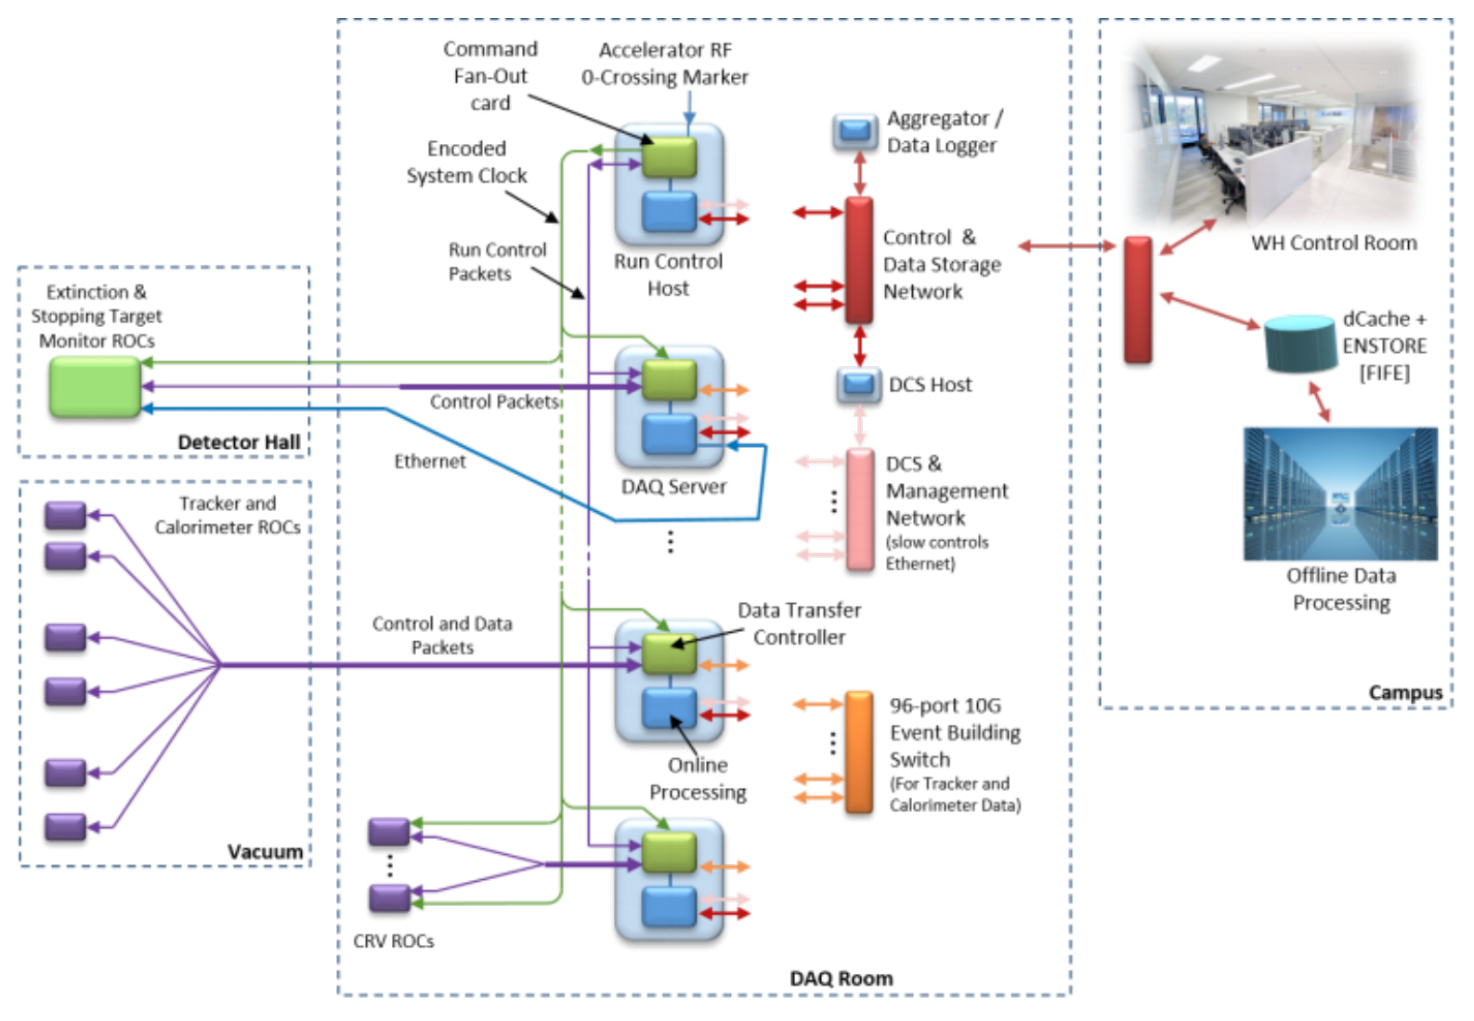
\includegraphics[width =\textwidth]{images/chapter2/Screenshot_20240206_144803.png}
\caption{Mu2e DAQ Architecture.}
\label{fig:linktodaq}
\end{figure}
The left blocks represent the Readout Controllers (ROCs) in different detectors. The center block houses the DAQ system's online components, which include the Run Control Host, 40 DAQ servers, the Detector Control System (DCS) and the Event Building Switch. The Run Control Host receives beam status and timing information from the Accelerator Controls network and operator commands from the remote control room. The Detector Control System (DCS) is the window onto the status and health of the Mu2e detector. The Event Building (EVB) function combines these subsets to form a complete detector data set for analysis by an online processor, Ref. \cite{bartoszek2015mu2e}. Event building is typically done in a switching network to sustain high rates. The right block houses the DAQ system's offline components, which are used for data storage and processing. During an active spill (the first approximately 43 ms of the 48 ms bunch extraction cycle outlined in Chapter \ref{accel}), the experiment receives RF Zero-Crossing Markers from the Accelerator that are synchronized to the 1695 ns proton pulse cycles (the event windows). Based on these markers, the Command Fan-Out (CFO) module within the Run Control Host generates a 40 MHz system clock and encodes Event Window Markers (EWMs) in the system clock to indicate the start of the event windows. The CFO then sends the encoded system clock, along with run control packets, to Data Transfer Controllers (DTCs) in the DAQ servers. The DTCs\footnote{The Mu2e Data Transfer Controller (DTC), Ref. \cite{ryan} takes data from various Read-Out Controllers and may conduct event construction and data preprocessing. The DTC module connects a maximum of six ROCs to the Trigger and Data Acquisition (TDAQ) servers, which execute the TDAQ online software framework.} then transfer the encoded clock to the detectors' ROCs, where the EWMs are recovered with fixed delay relative to the original RF Zero-Crossing Markers and used in the local ROCs to discriminate data acquired during consecutive event windows. The Tracker generates a DDR3 memory address at the beginning of each event window. The relevant memory area is designated to hold Tracker hits received during that event window. Data requests trigger data readouts from the ROCs to the DAQ system. The Data Requests are modifiable through the CFO as described by the Run Plan, although they are initially given to the Tracker and Calorimeter ROCs via the DTCs following each event window.

\subsection{TDAQ software: artdaq}





\subsubsection{Expected rate}





Each hit is composed of a data packet having a fixed length of 128 bits (16 bytes):
\begin{itemize}
    \item 16 bit header - it contains information as a packet header, a channel identifier to specify the channel so the ROC can assign the hit to a wire number and a packet checksum;
    \item 16 bit - TDC left straw end;
    \item 16 bit - TDC right straw end;
    \item 8$\times$10 bit ADC.
\end{itemize}
A packet of 128 bits can be transferred every 640 ns (200 Mbps).An additional 32
bits must be added as an end-of-file marker after the data $\mu$spill hit data is buffered.
The ROC-to-DAQ connection is made via fiber optic links arranged in rings, with multiple ROC per ring, as shown in Figure \ref{fig:linktodaq}. This is possible since a single optical link can handle 2.6 Gbps, while the ROC output is around 230 Mbps. This value comes from the fact that the highest rate for any 4 straws group (corresponding to one digitizer data line to the ROC) is 240 kHz or 30 Mbps (at 128 bits/hit) and the Main Injector supplies Mu2e beam only 32\% of the time. The ROC monitors slow control variables and controls panel operations too.


XXXXXXXXX: mettere le caratteristiche di Ref. \cite{vadi}  ?????

